%%% Local Variables:
%%% mode: latex
%%% TeX-master: t
%%% End:

\documentclass[type=master]{thuthesis}
% \documentclass[%
%   type=[bachelor|master|doctor|postdoctor], % mandatory option
%   secret,
%   openany|openright,
%   arialtoc,arialtitle]{thuthesis}

% 所有其它可能用到的包都统一放到这里了,可以根据自己的实际添加或者删除。
\usepackage{thuthesis}
\usepackage{url}

\newcommand{\tabincell}[2]{\begin{tabular}{@{}#1@{}}#2\end{tabular}}

% 你可以在这里修改配置文件中的定义,导言区可以使用中文。
% \def\myname{薛瑞尼}

\begin{document}

% 定义所有的eps文件在 figures 子目录下
\graphicspath{{figures/}}


%%% 封面部分
\frontmatter
%%% Local Variables:
%%% mode: latex
%%% TeX-master: t
%%% End:
%\secretlevel{绝密} \secretyear{2100}

\ctitle{多摄像头系统}
% 根据自己的情况选,不用这样复杂
\makeatletter
\ifthu@bachelor\relax\else
  \ifthu@doctor
    \cdegree{工学博士}
  \else
    \ifthu@master
      \cdegree{工学硕士}
    \fi
  \fi
\fi
\makeatother


\cdepartment[计算机]{计算机科学与技术系}
\cmajor{计算机科学与技术}
\cauthor{丁旭}
\csupervisor{陶品副教授}
% 如果没有副指导老师或者联合指导老师,把下面两行相应的删除即可。
% 日期自动生成,如果你要自己写就直接改这个cdate。
% 硕博也可以启用如下三行,替换其中的\the\year和\the\month为阿拉伯数字。
%\cdate{\zhdigits{\the\year}年\zhnumber{\the\month}月}

% 博士后部分
% \cfirstdiscipline{计算机科学与技术}
% \cseconddiscipline{系统结构}
% \postdoctordate{2009年7月——2011年7月}

\etitle{System}
% 这块比较复杂,需要分情况讨论:
% 1. 学术型硕士
%    \edegree:必须为Master of Arts或Master of Science(注意大小写)
%              “哲学、文学、历史学、法学、教育学、艺术学门类,公共管理学科
%               填写Master of Arts,其它填写Master of Science”
%    \emajor:“获得一级学科授权的学科填写一级学科名称,其它填写二级学科名称”
% 2. 专业型硕士
%    \edegree:“填写专业学位英文名称全称”
%    \emajor:“工程硕士填写工程领域,其它专业学位不填写此项”
% 3. 学术型博士
%    \edegree:Doctor of Philosophy(注意大小写)
%    \emajor:“获得一级学科授权的学科填写一级学科名称,其它填写二级学科名称”
% 4. 专业型博士
%    \edegree:“填写专业学位英文名称全称”
%    \emajor:不填写此项
\edegree{Master of Engineering}
\emajor{Computer Science and Technology}
\eauthor{Ding Xu}
\esupervisor{Associate Professor Tao Pin}
% 这个日期也会自动生成,你要改么?
% \edate{December, 2005}

% 定义中英文摘要和关键字
\begin{cabstract}
  论文的摘要是对论文研究内容和成果的高度概括。摘要应对论文所研究的问题及其研究目
  的进行描述,对研究方法和过程进行简单介绍,对研究成果和所得结论进行概括。摘要应
  具有独立性和自明性,其内容应包含与论文全文同等量的主要信息。使读者即使不阅读全
  文,通过摘要就能了解论文的总体内容和主要成果。

  论文摘要的书写应力求精确、简明。切忌写成对论文书写内容进行提要的形式,尤其要避
  免“第 1 章……;第 2 章……;……”这种或类似的陈述方式。

  本文介绍清华大学论文模板 \thuthesis{} 的使用方法。本模板符合学校的本科、硕士、
  博士论文格式要求。

  本文的创新点主要有:
  \begin{itemize}
    \item 用例子来解释模板的使用方法;
    \item 用废话来填充无关紧要的部分;
    \item 一边学习摸索一边编写新代码。
  \end{itemize}

  关键词是为了文献标引工作、用以表示全文主要内容信息的单词或术语。关键词不超过 5
  个,每个关键词中间用分号分隔。(模板作者注:关键词分隔符不用考虑,模板会自动处
  理。英文关键词同理。)
\end{cabstract}

\ckeywords{\TeX, \LaTeX, CJK, 模板, 论文}

\begin{eabstract}
   An abstract of a dissertation is a summary and extraction of research work
   and contributions. Included in an abstract should be description of research
   topic and research objective, brief introduction to methodology and research
   process, and summarization of conclusion and contributions of the
   research. An abstract should be characterized by independence and clarity and
   carry identical information with the dissertation. It should be such that the
   general idea and major contributions of the dissertation are conveyed without
   reading the dissertation.

   An abstract should be concise and to the point. It is a misunderstanding to
   make an abstract an outline of the dissertation and words ``the first
   chapter'', ``the second chapter'' and the like should be avoided in the
   abstract.

   Key words are terms used in a dissertation for indexing, reflecting core
   information of the dissertation. An abstract may contain a maximum of 5 key
   words, with semi-colons used in between to separate one another.
\end{eabstract}

\ekeywords{\TeX, \LaTeX, CJK, template, thesis}

% 设置 PDF 文档的作者、主题等属性
\makeatletter
\thu@setup@pdfinfo
\makeatother
% 如果使用授权说明扫描页,将可选参数中指定为扫描得到的 PDF 文件名,例如:
%\makecover[scan-auth.pdf]
\makecover

% 目录
\tableofcontents

% 符号对照表
%\begin{denotation}
\item[HPC] 高性能计算 (High Performance Computing)
\item[cluster] 集群
\item[Itanium] 安腾
\item[SMP] 对称多处理
\item[API] 应用程序编程接口
\item[PI] 聚酰亚胺
\item[MPI] 聚酰亚胺模型化合物,N-苯基邻苯酰亚胺
\item[PBI] 聚苯并咪唑
\item[MPBI] 聚苯并咪唑模型化合物,N-苯基苯并咪唑
\item[PY] 聚吡咙
\item[PMDA-BDA]	均苯四酸二酐与联苯四胺合成的聚吡咙薄膜
\item[$\Delta G$] 活化自由能~(Activation Free Energy)
\item [$\chi$] 传输系数~(Transmission Coefficient)
\item[$E$] 能量
\item[$m$] 质量
\item[$c$] 光速
\item[$P$] 概率
\item[$T$] 时间
\item[$v$] 速度
\item[劝 学] 君子曰:学不可以已。青,取之于蓝,而青于蓝;冰,水为之,而寒于水。木
  直中绳。輮以为轮,其曲中规。虽有槁暴,不复挺者,輮使之然也。故木受绳则直,金就
  砺则利,君子博学而日参省乎己,则知明而行无过矣。吾尝终日而思矣,不如须臾之所学
  也;吾尝跂而望矣,不如登高之博见也。登高而招,臂非加长也,而见者远;顺风而呼,
  声非加疾也,而闻者彰。假舆马者,非利足也,而致千里;假舟楫者,非能水也,而绝江
  河,君子生非异也,善假于物也。积土成山,风雨兴焉;积水成渊,蛟龙生焉;积善成德,
  而神明自得,圣心备焉。故不积跬步,无以至千里;不积小流,无以成江海。骐骥一跃,
  不能十步;驽马十驾,功在不舍。锲而舍之,朽木不折;锲而不舍,金石可镂。蚓无爪牙
  之利,筋骨之强,上食埃土,下饮黄泉,用心一也。蟹六跪而二螯,非蛇鳝之穴无可寄托
  者,用心躁也。\pozhehao{} 荀况
\end{denotation}



%%% 正文部分
\mainmatter
\chapter{引言}


\section{研究背景}

随着互联网技术的不断发展,社交网络已经成为人们日常生活中不可或缺的一部分。人们可以通过社交网络获取新闻,与他人进行交流互动,发布个人信息等等。对于大多数中国互联网用户来说,QQ、微博、微信、陌陌等社交应用是其日常上网的主要应用。根据中国互联网络信息中心(CNNIC)的调查结果显示\cite{internetSurvey},有79.5\%的用户每天上网的时间达到两个小时以上,而其中77.0\%的时间是用在社交应用上。社交网络使得人们不再受报刊、电视等信息来源的限制,拥有了更多获取信息的渠道。

\begin{figure}[h] 
  \centering
  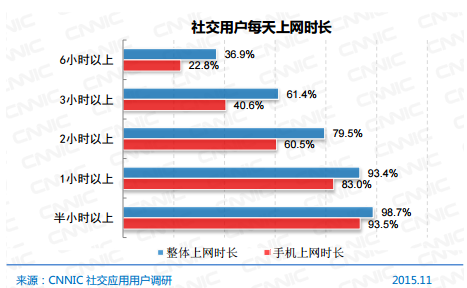
\includegraphics[height=8cm]{InternetUsingTime}
  \caption{社交用户每日上网时长\cite{internetSurvey}}
  \label{InternetUsingTime}
\end{figure}

对于信息发布者来说,社交网络给他们提供了一个新的推广和营销平台。由于大量用户花费大量时间在社交网络中,传统的信息发布渠道日渐衰落,而社交网络凭借其传播范围广、扩散速度快、受众数量大、推广形式多等特点,逐渐成为一种全新的、重要的、高效的推广方式。Shama Hyder在《网络社交媒体营销》一书中提到社交媒体必将取代传统媒介成为营销推广的主要手段 \cite{hyder2016zen}。

利用社交网络进行推广营销,能够在短时间内将信息传递给目标群体。在微博、微信公众号等社交平台上,流行用户往往拥有几百万甚至几千万的关注量,其发布的每一条消息都有大量的用户关注。且传播速度快,实时发送接收,还能够根据受众的不同发布不同的信息,使得推广行为更加具有针对性。同时,利用社交网络进行推广,形式上更加灵活多样,利用文字、图片、语言、视频的手段,能够更加充分地进行展示。优秀的推广内容甚至能够通过用户自发进行传播,呈现爆发式营销增长。著名社交网络公司Facebook,在2016年广告业务的总收入达到268亿美元\cite{Facebook}。而微博在2016年Q4季度中,其广告收入也达到了1.879亿美元\cite{微博}。这仅仅是这两家社交网络公司自身的广告营销收入,其最大的贡献是为其用户提供了一个社交网络的营销平台,由此产生的推广营销效益更加巨大。

由于社交网络推广方式的灵活性,对于商品、活动、人物等众多对象均可以进行推广,本文主要研究的是演员针对影视剧在社交网络上的推广。影视剧的关注人群广泛,且娱乐性、话题性强,能够更好地适用于社交网络上的多种推广模式。

随着大数据、机器学习等技术的不断进步,社交网络在影视剧推广方面的重要作用越来越不容忽视。以著名的国产电影《失恋33天》的社交网络营销为例,该部电影在2011年上映,凭借成功的网络营销手段,取得3.5亿人民币的优秀票房,是原预估票房的十倍以上\cite{熊莉2012失恋}。在2011年的11月16日,通过百度搜索引擎搜索“失恋33天”关键字,能够找到相关结果约394万个,在谷歌搜索“失恋33天”,能够找到约5900万个相关结果。在社交网站微博上搜索“失恋33天”能够找到约670万条消息,在腾讯微博上,则能够搜索到330万条消息\cite{熊莉2012失恋}。

\begin{figure}[h] 
  \centering
  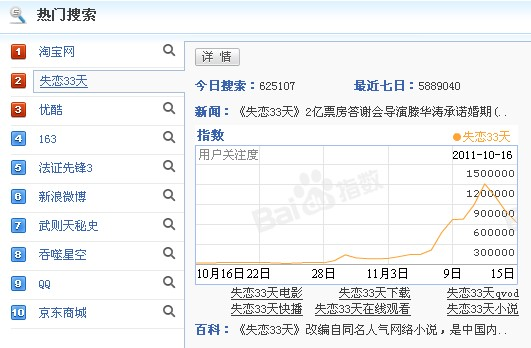
\includegraphics[height=8cm]{失恋}
  \caption{《失恋33天》百度搜索结果}
  \label{失恋}
\end{figure}

这部电影以新浪微博、腾讯微博等社交网站为重要推广平台,打造了拥有近10万粉丝量的官方微博,并创建了众多热门话题,通过宣传短片、制造话题等众多手段,针对网络用户的特点精准投放营销策略,并引导用户参与话题讨论,通过转发、评论等手段,将用户自身的社交网络融入到宣传网络当中,进一步扩大了宣传效果。在日后的各类总结点评中,《失恋33天》都被认为是电影营销手段的一次最成功的创新,利用社交网络对影视剧进行推广的方法从此日益发展。

通过对现有社交网络推广案例进行分析即可发现,目前针对影视剧的网络营销手段层出不穷,而且还存在着继续增多的趋势。例如宣传方会在微博、QQ、微信等社交媒体上创建官方账号,发布关于影片的文字、图片消息,演员消息,宣传短片等。这样的宣传方式会在影片上映前后持续较长时间,吸引大量粉丝关注,提高影片关注度。例如最近上映的电影《嫌疑人X的献身》,其在微博上的官方账号共发布了744条微博,拥有62万粉丝关注,发布的每条微博有数千条的转发、评论、点赞\footnote{http://weibo.com/p/1002065746403567}。

\begin{figure}[h] 
  \centering
  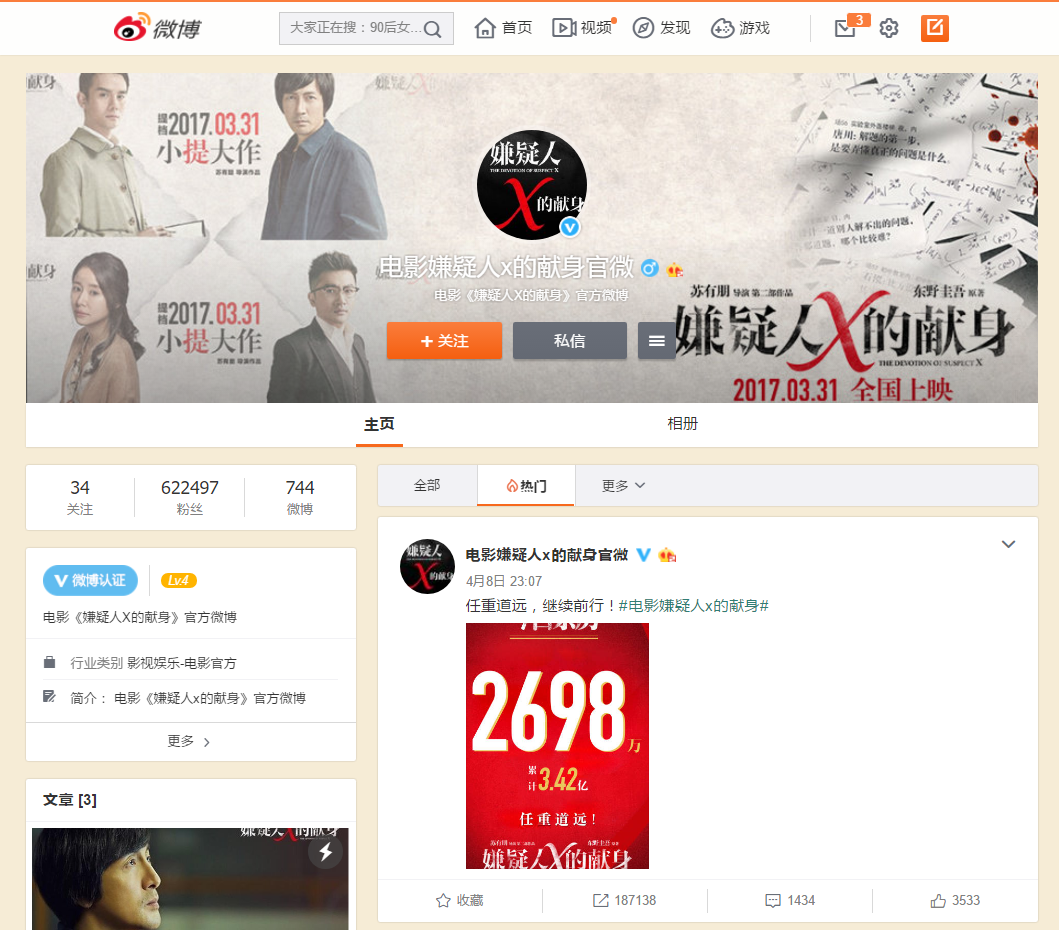
\includegraphics[height=10cm]{嫌疑人}
  \caption{《嫌疑人X的献身》官微截图}
\end{figure}

同时,宣传方还会在社交网络上制造影视剧相关话题,并不断推高话题热度,扩大影片影响力。例如电影《致青春》在网络营销中通过推出“回忆青春”、推出主题曲、制造“有一种感情叫赵薇黄晓明”等流行语的形式制造多个热点话题,激发用户自动传播,最终实现病毒式传播效果。另外宣传方还可以通过各类影评、新闻报道提升观众的观看热情。例如最近热播的电视剧《人民的名义》在豆瓣网可以找到近4万篇影评\footnote{https://movie.douban.com/subject/26727273/},短短一周之内在微信公众号上即出现了55篇与其有关的阅读量超过10万的文章,这样的推广方式能够为影视剧打造良好的口碑,塑造良好形象,吸引更多观众观看。

而网络推广的各种营销手段,往往是通过一些关键节点传播和扩散给广大用户,这些节点一般是由影视剧的官方账号、演员或者经过社交平台验证的“大V”用户组成。这些用户拥有巨大的粉丝量,能够将各类宣传消息推送给众多的用户,起到宣传媒体的作用\cite{kwak2010twitter}。

影视剧演员往往拥有众多粉丝,关于演员的新闻报道和演员自身发布的消息都能够获得极高的关注度,演员在社交网络中具有较高的影响力\cite{shafiq2013identifying},是影视剧宣传推广的重要节点。影视剧演员可以通过自身的影响力在社交网络上制造话题,通过发布各种类型的消息,包括文字、图片、音视频等等,或者利用其它用户发布关于自己的新闻报道,即可以引起关注自己的粉丝的广泛反响,引发热烈讨论。然后根据网络话题演化的规律\cite{he2009detecting},在适当时刻不断推高话题热度,使其成为热点,获得更多受众。因此,在对影视剧进行宣传的过程中,演员就可以利用其巨大的影响力,制造并推动关于影视剧的相关话题,引起其在社交网络中的广泛关注,对影视节目的宣传推广起到重要的促进作用。

但是在进行推广时,不同的推广方式会收到不同的推广效果,不同的用户使用同样的推广方式也会得到不同的结果。如图~\ref{蒋欣}所示,演员蒋欣在对其主演的电视剧《欢乐颂》进行宣传时,发布了两条微博,但是其转发和点赞数量却有很大的不同。可想而知,这两条微博能够获得的推广效果也是截然不同的。

\begin{figure}[h]
  \centering%
  \subcaptionbox{转发:7186 评论:25817 点赞:143036}
    {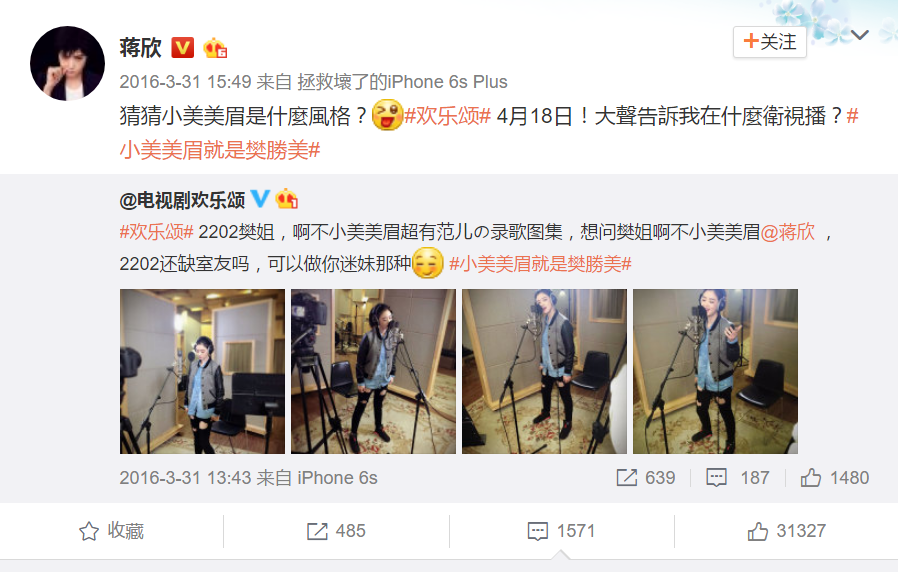
\includegraphics[height=4.5cm]{蒋欣1}}
  \subcaptionbox{转发:485 评论:1571 点赞:31327}
      {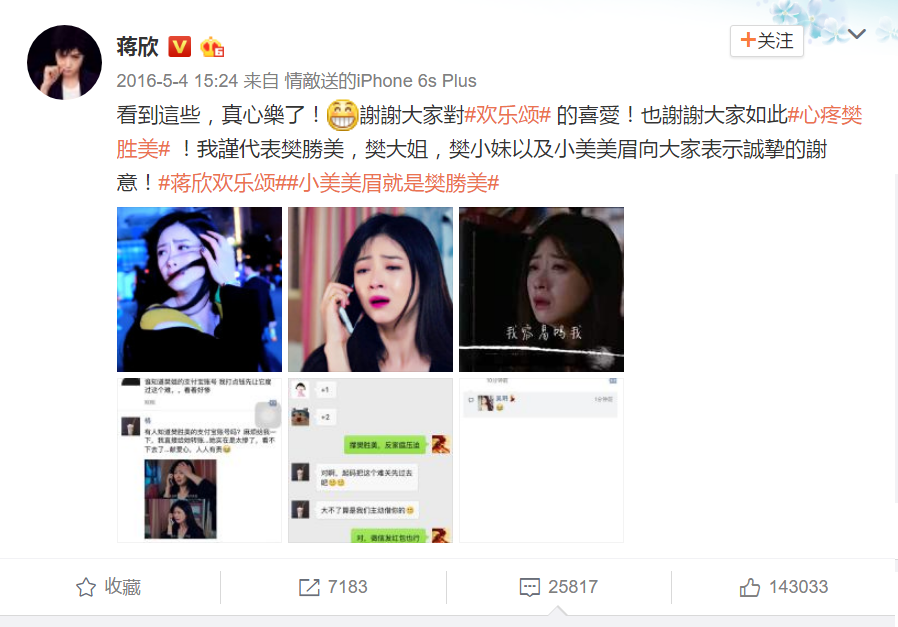
\includegraphics[height=4.5cm]{蒋欣2}}
  \caption{不同微博的推广效果比较}
  \label{蒋欣}
\end{figure}

另外,对电影和电视剧的推广有很大差异。例如,对于电影的推广来说,由于其属于一次性消费,只需要吸引观众进入影院观看即可。而对于电视剧的推广来说,由于其播放周期较长,需要对用户维持长时间的粘滞力,在吸引新用户进行观看的同时,还有保持老用户的持续关注。因此,对于电影和电视剧的推广手段就需要有不同的侧重点,需要有针对性地采用不同的推广方式。目前关于电影推广的研究较为常见,由于电影的高投入高产出性,宣传方也会投入更多精力关注电影推广。而关于电视剧有针对性的推广研究较少,推广方式也较为有限,需要给予更多的关注。

因此,为了能够获得更好的推广效果,最大限度地发挥社交网络的推广作用,本文选取演员在社交网络上的对于电视剧的推广微博作为研究对象,根据演员自身和待推广电视剧的特点,分析不同推广策略带来的不同的微博影响力,识别出最有效的推广策略。

\section{主要研究内容和挑战}

本文的数据来源是爱奇艺、豆瓣和微博,获得电视剧相关、演员相关的所有基本信息和社交行为信息,如电视剧官方微博数据、电视剧话题数据、演员粉丝量、演员发布的所有微博信息等等,并对这些数据进行了整理和分析。

首先针对这些数据进行了一些测量,比如基于粉丝参与度(微博转发量、评论量、点赞量)提出微博影响力指数,来衡量一条微博能达到的推广效果,进而能获得演员发布关于电视剧的微博的总体微博影响力;测量电视剧微博话题热度与微博影响力之间的相关性,静态数据和动态数据都说明了二者的高度相关性,从而利用微博影响力来刻画能达到的话题热度,等等。

然后从数据中识别出演员发布电视剧相关微博的推广模式,包括演员在电视剧不同时期的推广特点,不同时间的推广特点,发布形式上的互动特点等,其中还包括一些推广规律,如虽然有很多演员在微博上并不活跃,但是几乎所有演员都会在电视剧上映前几天发布推广微博;发现大部分演员都在很短的时间内对官微“@”自己的微博进行响应等等。

最后利用倾向值匹配模型对演员在社交平台上的推广行为进行分析建模。对各个推广策略与推广效果之间的因果关系一一进行分析,识别电视剧推广的最有效的策略。并且在这个过程中不断进行优化,在应用模型时引入了更多的混淆变量,更充分的考虑各种会影响推广效果的因素,同时结合电视剧话题在微博上的演化规律,对演员的推广行为进行分段处理,更精准更合理地识别有效策略。另外,还对模型进行了显著性检验和平衡性检验,验证了该模型的适用性和准确性。

本文所述研究主要存在如下几方面挑战:

\begin{itemize}

\item[(1)]目前基于社交媒体数据的研究主要集中在电影领域,关于电视剧的研究较少,且关于电影的研究主要是结合社交数据进行票房预测,很少集中在推广领域。同时,电影是一次性消费,而电视剧是一个持续性消费,除了首播前的宣传,当电视剧开播后,在维持现有观众群、防止用户流失的同时还要吸引更多人来观看。关于电视剧在社交网络上的推广行为的研究更是少有相关工作可以参考,但是微博作为电视剧推广的重要平台,好好利用能达到事半功倍的效果。

\item[(2)]理想情况下,检验策略有效性的黄金标准是基于实验的方法,比如做A/B测试,但是随机对照实验成本高,随机选取用户随机分配策略操作性非常低,实际环境中不可实现。因此提供一个基于观测数据的统计方法而不是实验方法来检测策略的有效性是非常重要和有必要的。

\item[(3)]采用非随机对照实验的方法容易出现数据偏倚、组间基线不齐,即结果会受混淆变量的影响。在考虑到各个混淆变量的情况下,如何排除混淆变量的影响,得到推广策略和推广效果之间的净效应也是一个难点。如直接选用回归关系,一是推广策略与推广结果不一定是线性关系,二是混淆变量可能与推广策略和推广结果都有关系,可能有共线性问题。

\item[(4)]数据获取难度大。首先是微博整体用户量大,跟电视剧相关的微博量大而难以全量获得,研究所有用户的数据比较困难。然后是根据电视剧基本信息如何对应到电视剧和演员在微博中id,以及获得id后如何在非好友、无权限的情况下爬取他们的全量数据,都是有待解决的问题。


\end{itemize}

\section{主要贡献和组织结构}

针对以上的问题与挑战,本文选取演员发布的微博作为研究对象,更有代表性和针对性,利用倾向值匹配模型,将混淆变量纳入Logistic模型,归纳成一个倾向值,进行倾向值匹配时,用以控制混淆变量,使得对最终结果的影响只能归因于自变量,从而有效评估出演员推广电视剧的有效策略。本文的主要贡献如下:

\begin{itemize}

\item[(1)]基于社交媒体数据的影视剧研究领域,更多的是对于电影的关注,由于电视剧播出周期长、用户行为复杂等问题,电视剧相关的研究往往被忽略。而本文以电视剧推广作为研究目标,分析演员在微博上对电视剧的推广行为,有效填补了这方面研究的空白。而且微博已成为电视剧推广不可或缺的平台,演员在电视剧的宣传过程中起到了信息专家和中心节点的作用,吸引粉丝参与话题讨论,促进话题热度提高,分析他们的推广行为具有重要意义。

\item[(2)]本文利用倾向值匹配模型对演员在社交平台上的推广行为进行分析建模。不但解决了随机对照实验成本高、操作性低等问题,还解决了可能出现的选择偏倚、混淆变量影响等问题。对各个推广策略与推广效果之间的因果关系一一进行分析,排除混淆变量的影响,分析推广策略与推广效果之间的净效应,识别电视剧推广的有效策略。还对模型进行了显著性检验和平衡性检验,验证了该模型的适用性和准确性。而且在以往的研究中,倾向值匹配算法多用于医药学、社会学和经济学等领域,在社交媒体大数据领域的应用较少,本文的应用开拓了一种新的应用方向。

\item[(3)]本文不但做了一些基本测量,可以指导未来研究,如基于粉丝参与度提出微博影响力指数,利用静态数据和动态数据说明话题热度与微博影响力的相关性等;还发现了一些推广模式和推广规律,如一种常见推广模式是电视剧官方微博作为话题的源头来发布微博,同时"@"其他演员,然后其他演员通过转发微博来响应官微,来扩大微博影响力,同时发现大部分演员对官微的响应都在很短的时间内等。

\item[(4)]本文结合了电视剧话题在微博上的话题演化规律进行综合分析,对演员的推广行为进行分段研究,更精准更合理地识别有效策略。因为在电视剧的不同时期,演员的推广特点和推广侧重点有所不同。在电视剧拍摄期间,演员会发布电视剧拍摄相关的信息如拍摄进度、角色定妆照等,电视剧首映前,演员会发布微博提醒粉丝们电视剧的首映时间,电视剧上映时,他们会发布更多的微博讨论电视剧角色、剧情等。因此,对演员的推广行为进行分段研究更具有指导意义。

\item[(5)]为了避免获取全部微博数据产生的海量数据,本文选取演员发布的推广微博作为研究对象。不但使研究更有代表性和针对性,还有效降低了实验数据量。在数据获取过程中,采用多种方法和技术获取数据,包括模拟搜索、模拟登陆、抓取手机端数据而非电脑端数据等方法,解决了非好友、无权限下无法获取数据和获取速度慢的问题。

\end{itemize}

本文的组织结构如下:

第二章主要介绍研究现状和相关工作,包括当前关于影视剧和社交网络相结合的研究情况,因果分析的主要研究方法,以及基于倾向值匹配的因果分析方法的发展和应用情况。

第三章主要介绍本文所使用的实验数据集,包括数据的来源、收集方法和数据形式。同时还介绍了基于该数据集进行的一些基础分析、测量和从中挖掘出的数据特征和规律等。

第四章主要介绍了倾向值匹配算法的原理、具体算法步骤以及对模型的验证方法。

第五章将倾向值匹配算法应用到数据集上,对不同的推广策略进行了比较分析,并提出了一种改进模型,验证了该算法对推广策略分析的适用性和准确性。

第六章是对全文的总结,以及对下一步工作的展望。





































\chapter{研究现状和相关工作}

\section{本章引言}

本章首先介绍了多摄像头系统的发展现状以及发展趋势,并列举了若干多摄像头系统的性能以及实现方法。然后介绍了对摄像头拍摄时间进行检测的相关方法。最后介绍了多摄像头系统同步控制的几种方法,主要可以分为硬件控制和软件控制两大类。

\section{多摄像头系统}

多摄像头系统一般由多个单一摄像头组合而成,包括数据采集、控制、数据存储分析等几部分。多摄像头系统的优势在于融合了各个摄像头的优点,并且利用数量上的优势成倍将这些优点放大。如果需要满足多种拍摄要求,就需要摄像头满足多种性能指标,对于单一摄像头来说大多数情况下很难满足这些要求,而能够满足要求的摄像头往往较为昂贵或难以获得,甚至有些情况下对于摄像头的多种性能要求是相互矛盾的,根本无法实现。但是多摄像头系统就能够很好地解决这一问题,多摄像头系统可以利用多个具有不同性能指标的摄像头,选取所需的功能进行融合以满足要求。同时还可以利用多个摄像头的融合使其性能指标大幅增长,从而利用廉价摄像头实现了高品质摄像头的功能。

目前多摄像头系统主要可分为两种类型,一类是大规模同类摄像头集成,一类是异种摄像头组合搭配。同类摄像头集成一般采用较多的相同性能参数摄像头组成摄像头阵列,以形成规模优势。Stanford大学计算图形学实验室搭建了一个多摄像头阵列 \cite{3},就是利用了低成本摄像头的价格优势和高性能处理器的运算优势,将100个CMOS图像传感器数码摄像头组成阵列形式。每个摄像头由两部分组成,一部分负责图像采集,由互补金属氧化物半导体(CMOS)图像传感器和廉价镜头组成,一部分负责数据处理,由视频编码器、现场可编程逻辑门阵列(FPGA)和IEEE 1394(Firewire)传输接口组成。该多摄像头系统能够对100个摄像头拍摄到的视频进行实时同步压缩,并将数据保存在硬盘中。

\begin{figure}[h] 
  \centering
  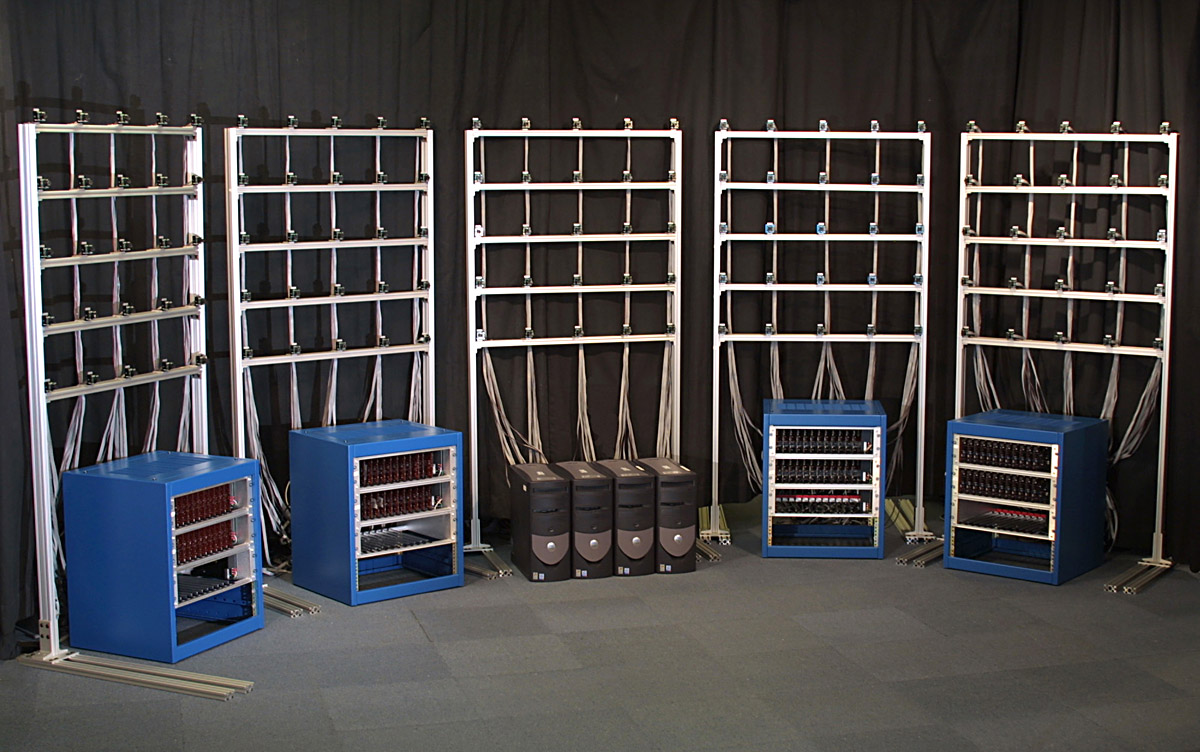
\includegraphics[height=6cm]{Stanford2}
  \caption{Stanford大学多摄像头阵列}
  \label{Stanford2}
\end{figure}

根据各个摄像头排列方式和拍摄角度的不同,该多摄像头系统能够实现多种功能。当各个摄像头紧密排列时,可以将系统视为一个单中心的合成相机,将各个摄像头拍摄到的数据进行合成处理后,就能够大幅度提升各项性能参数,如动态范围、景深、帧率和光谱灵敏度等 \cite{4, 7}。当各个摄像头排列间隔较远时,可以将该系统视为多中心摄像机,即为视场相机。通过该视场相机可以应用新的三维场景重建方法以及多视角全景构建方法 \cite{5}。当各个摄像头间隔排列时,可以将系统视为一个大合成孔径相机,使得该系统可以通过部分闭塞的环境观察拍摄对象,即实现共聚焦镜头的离散近似,使得不在选定平面上的物体变得模糊和黑暗 \cite{6, 8}。

Parziale等人在文献 \cite{parziale2006surround} 中设计了一种利用多摄像头系统,在非接触条件下检测人手指纹的装置。为了避免在恶劣条件下通过按压方式提取指纹时产生的误差,该系统利用五个小型摄像头多角度对手指进行拍摄,并通过图像处理提取指纹信息,有效避免了因皮肤过于干燥或存在过多水分等因素对指纹检测造成的影响,实现了小型化高准确度的指纹检测系统。

同时,利用多摄像头系统进行视频监控也是一个广泛的应用场景。文献 \cite{taj2009multi, bellotto2009distributed, fiore2008multi, kettnaker1999bayesian} 中分别介绍了利用多个摄像头在不同应用场景下组成多摄像头监控系统,通过硬件配置和软件优化,监控探测多种对象。

另一类多摄像头系统由不同性能的摄像头组合而成,这样可以充分发挥各个摄像头的性能优势,从而满足使用者对于系统的多种需求。例如在欧洲航天局(ESA)和俄罗斯联邦航天局合作推动的火星探测计划(ExoMars)中 \cite{9, 10},为了能够使火星登陆车实现周边地形勘测、火星车自身定位、大气及周边环境监测、科学实验观测等功能,研究人员将配置在火星车上的全景摄像头(Panoramic Camera)设计成了一个多摄像头系统。该系统是由一个高分辨率摄像头(HRC)和两个广角立体摄像头(WAC)组成。其中高分辨率摄像头的有效像素为1024 × 1024,主要负责细节图像的拍摄。而广角立体摄像头配备视角为65°的镜头,通过两个摄像头采集到的图像进行融合,模拟人眼实现立体成像,主要负责观测周围环境。这样,该系统通过不同性能指标的摄像头之间的配合,实现了所需的全部功能。

\begin{figure}[H] 
  \centering
  \includegraphics[height=6cm]{Mars}
  \caption{火星登陆车上的全景摄像头}
  \label{Mars}
\end{figure}

最近一段时间,多摄像头系统也被广泛应用于智能手机的摄像头模块上。Apple公司推出的最新手机iPhone 7 Plus就配备了双目摄像头模块 \cite{iphone},由广角和长焦两颗摄像头组成,广角摄像头主要负责近景拍摄,而长焦摄像头主要负责远景拍摄,从而相互配合实现光学变焦功能。华为公司推出的P9手机同样配备双摄像头系统,但是两颗摄像头分别为黑白和彩色摄像头 \cite{华为},黑白摄像头负责捕捉景物细节,使得成像更为清晰,而彩色摄像头负责捕捉颜色,使得图片色彩更为饱满,通过对不同摄像头拍摄到的图像的算法融合,得到更好的拍摄效果。

\begin{figure}[h]
  \centering%
  \subcaptionbox{iPhone 7 Plus}
    {\includegraphics[height=5cm, width=6.5cm]{iphone}}
    \hspace{4em}%
  \subcaptionbox{华为 P9 手机}
      {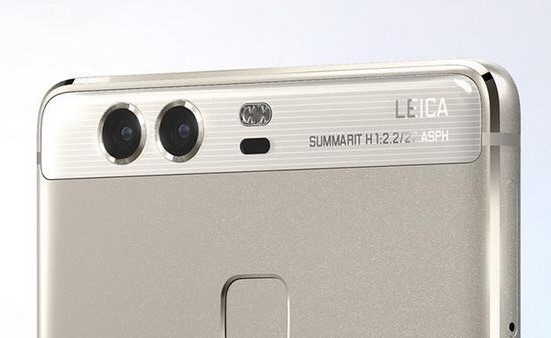
\includegraphics[height=5cm, width=6.5cm]{华为}}
  \caption{智能手机上的多摄像头系统}
\end{figure}

除了对于多摄像头系统组成搭建方法的研究,目前还有部分研究是围绕多摄像头系统拍摄视频内容的分析展开。例如针对视频内的运动物体进行追踪,在安防监控等领域有较多应用。Ting-Hsun Chang等人在文献 \cite{11} 中提出了一种基于贝叶斯模态融合的方法,利用多摄像头系统追踪室内环境下多个人的移动轨迹。为了连续追踪运动物体,该系统为每个新检测到的对象设定特有的模式,当对象移动或进入到其他摄像头视野内时,系统会利用贝叶斯网络组合匹配各个模式,以实现连续追踪。不同于其他单一摄像头的闭塞推理追踪方法,该方法利用多摄像头系统进行交互追踪,能够大大提高追踪精度。同样Kim等人在文献 \cite{12} 中也提出了一种基于平面跟踪对应模型(TCM)的方法来对大规模多摄像头系统内的对象进行跟踪。该方法为每个运动对象计算了一个唯一且不变的追踪对应模型,使得在不同摄像头的视野内,或者在各个摄像头重叠的视野内,对于同一个物体来说有且只有一个追踪对应模型,这样就能能够准确追踪对象的运动。文献 \cite{zha2013detecting, saini2014w3, wang2013intelligent} 分别介绍了利用多摄像头系统进行对象检测或跟踪的方法。

还比如针对拍摄图像进行多摄像头校准,以实现更好的拍摄效果。Strecha等人在文献 \cite{13} 中为了实现基于图像的三维建模技术,需要将各个摄像头进行校准并实现多角度立体视觉。Baker等人在文献 \cite{14} 中为了校准各个摄像头,利用LED灯光建立点对(point correspondences),输入到大规模非线性特征值最小化程序当中,使得各个摄像头两两之间建立全息投影矩阵。Kurillo等人在文献 \cite{15} 中提出了一种广域校准方法,利用LED灯光标识作为校准对象,利用矩阵分解计算摄像头初始姿态,并通过自动构建加权视觉图,同时在相机之间找到最佳的变换路径来解决全局校准。文献 \cite{theriault2014protocol, knorr2013online, heng2014infrastructure} 分别利用图像内的地面、基础设施等参照物对多路摄像头图像进行校准。

另外一些研究是针对多摄像头拍摄结果进行拼接。Hongming Zhang等人在文献 \cite{16} 中为了解决前景对象在视频拼接过程中造成的割裂问题,提出了一种前景对象边缘调整的方法。该方法将各个摄像头拍摄到的图像进行前景提取,并根据前景图像的内容动态调整拼接边缘,再对于静态的背景图像进行拼接,最后将前景图像与背景图像进行融合即可得到拼接结果。文献 \cite{malesa2014multi, zhong2014color, lu2016photometric} 中也介绍了更多的多摄像头图像拼接方法,图像拼接技术在众多领域都有着广泛而深入的研究和应用。

\section{摄像头拍摄时间检测}

对于一个同步的多摄像头系统而言,其中各个摄像头的拍摄时间是由系统内部时间确定的,系统会给每张图像打上时间戳用以确定系统同步精度。但是由于在多摄像头系统内可能存在的网络传输延时、硬件信号处理延时、程序运行延时、系统时间漂移等因素,会导致图像时间戳与摄像头实际的曝光时间存在一定的差异,这个差异就是系统的同步误差。因此在利用时间戳作为摄像头拍摄时间检测标准的基础之上,还需要更加准确的方法来检测摄像头的拍摄时间。

戴琼海等人在文献 \cite{戴琼海111} 中利用多个LED灯显示串行时间码IRIG-B信号。外部触发控制器控制LED灯开始显示,并在同一时刻向摄像机发送拍摄信号。则摄像机的曝光开始时间与LED灯的显示时间相同,拍摄到的图像中LED灯显示的时间即为摄像机的拍摄时间。此方法的不足之处在于需要外部控制其进行控制,要求摄像机具有接收控制信号的硬件接口。同时由于系统延时无法保证摄像机曝光开始时间与显示时间精确相同。

赵莉等人在文献 \cite{赵莉1992高速摄影机数据记录系统研究} 中利用LED点阵显示二进制整数表示时间,当摄像机拍摄到点阵后即可确定时间。由于点阵显示不断变化,为了避免摄像机拍摄到多个显示的时间产生重叠,该方法需要设定点阵中LED灯的亮灭变化周期不大于要求的检测精度,同时摄像机曝光时间不大于此变化周期,但是当曝光周期处于两个显示时间之间时,仍有可能拍摄到时间叠加。而且当要求检测精度较高时,曝光时间也相应变短,从而导致拍摄到的图像曝光不充分或者曝光时间过短摄像机性能无法满足需求。

Qi Zhao等人在文献 \cite{zhao2009high} 中利用单一LED灯作为信号源,控制其亮灭变化满足独立同分布。使用多个摄像机对其进行拍摄并将拍摄结果根据亮灭分布进行匹配,从而计算各摄像机之间的相对时间偏差。该方法需要多个摄像机长时间拍摄才能够达到较高检测精度,检测灵活性较低。


\section{多摄像头系统的同步控制}

多摄像头系统的同步控制,其主要的目的是为了能够精确控制系统内各个摄像头的拍摄时间,以减小拍摄时间误差对拍摄结果造成的影响。例如,当利用多个摄像头从不同角度拍摄某一对象时,如果该对象静止不动,则各个摄像头的拍摄时间即使存在误差也不会影响拍摄结果。但是如果该对象是在不断变化,则各个摄像头会在不同时刻拍摄到该对象的不同状态,如果各个摄像头之间并非精确同步,其拍摄时间存在一定波动,那么就无法拍摄到同一时刻该对象的相同状态。同样,当利用多个摄像头按照一定的时间间隔,在不同时刻连续拍摄某一对象的变化,如果各个摄像头之间并非时间同步,那么就无法控制其按照设定好的时间间隔拍摄,可能会发生拍摄时间的重叠、提前或延后。

现阶段,对多摄像头系统进行同步控制,主要分为硬件同步和软件同步两种。利用硬件进行同步时,需要通过特殊的硬件接口,如IEEE-1394接口、Camera Link接口等,将系统内各个摄像头连接到一起,通过控制器发送控制信号给摄像头。而利用软件进行同步时,则是根据拍摄到的图像数据分析拍摄时间从而对各个摄像头进行调整。

\subsection{硬件同步}

硬件同步控制主要可分为两类:一类是利用多路图像数据采集卡实现,一类是利用外部触发信号源实现。

图像数据采集卡是一种对摄像头图像数据进行获取、处理、存储等功能的硬件设备。通过硬件接口与摄像头进行连接,接口的种类包括模拟接口,如AV接口、S端子等,和数字接口,如PCI总线、USB接口等。图像数据采集卡一般都集成了对摄像头的控制模块、编解码模块、存储模块等功能模块,因此具有多个输出接口的采集卡能够对多路摄像头进行控制。在图像数据采集卡的使用过程当中,一般对于摄像头的要求较高,需要摄像头具有专门的通信接口能够同采集卡进行连接,并且能够对采集卡的控制信号做出响应,同时也要保证采集到的数据能够被采集卡所识别。虽然采用图像数据采集卡能够在硬件层面对多路摄像头进行比较精确的同步控制,但是由于此类采集卡多为成熟产品,开放程度较低,难于对其进行更底层的控制,同时对于摄像头的要求限制也较多,其应用场景并不广泛。

目前市面上可以购买的图像数据采集卡种类很多,其主要差别在于摄像头接口种类、输出接口数量以及其他一些附加功能。同样也有很多关于设计并实现多路图像数据采集卡的研究。如朱海宽等人在文献 \cite{17} 中设计并实现了一种基于PCI总线的多路图像采集卡;刘晓军等人在文献 \cite{刘晓军2009采用} 中实现了一种具有HD-SDI高清串行数字接口的FPGA视频采集卡;王剑飞等人在文献 \cite{王剑非2007基于} 中实现了在Linux平台下的视频采集设备的驱动程序。

为了消除图像数据采集卡在使用过程中的种种限制,更多的多摄像头系统采用外部触发信号源实现同步控制功能。这类系统内的各个摄像头都具有触发信号的收发接口,通过接口与控制器相连接,控制器根据系统需求在特定的时刻发送触发信号给各个摄像头。姜广文等人在文献 \cite{姜广文} 中提出了一种基于外触发的多摄像头同步系统的设计方法。该方法采用USB接口的数字输出模块作为同步触发信号发生器,将高精度的触发信号发送给各个摄像头,实现同步功能。国蓉等人在文献 \cite{国蓉2014具有} 中利用同步信号发生器和锁相环电路实现同步功能。当摄像头接收到同步触发信号后,开始进行曝光拍摄。经试验验证,触发信号与摄像头拍摄周期之间的相位差为10度,远小于摄像头的曝光时间间隔。在文献 \cite{Prochazka} 中,多摄像头系统中的所有摄像头通过IEEE-1394总线节点连接,并通过控制器自动对摄像头进行控制,该系统的最小控制误差为125\textmu s。但是由于IEEE-1394总线的性能限制,每个节点能够控制的摄像头有一定的数量限制,并且不同总线之间的同步需要额外的同步单元,实现较为复杂 \cite{Litos}。Zitnick等人在文献 \cite{Zitnick} 中利用两个集线器(concentrators)来控制8个摄像头,并利用FireWire火线接口将两个集线器进行同步,系统实现更为复杂。同时,还有一些多摄像头系统利用GPS等通用信号进行同步,这样同步信号全局分发,可以有效消除误差。如黄芳等人在文献 \cite{黄芳} 和刘团结等人在文献 \cite{刘团结} 中所介绍的方法都利用的GPS信号进行同步。但是这些方法往往对于系统和摄像头的性能、接口要求较多,且要能够保证实时接收同步信号,实现难度较大。

\subsection{软件同步}

利用硬件进行多摄像头同步时,往往要求摄像头具有特定的硬件接口以实现同步信号的接收,这就使得大多数日常生活中接触到的普通摄像头无法应用这种方法进行同步,给多摄像头系统搭建提出了更高的硬件要求。而软件同步是利用各个摄像头拍摄到的数据,通过分析视频内容确定拍摄时间或者各个摄像头之间的时间间隔,从而实现同步控制功能,因此对于摄像头并无更多的硬件接口要求,适用的范围更加广泛,应用场景更多。

软件同步也可以主要分为两类,一类是利用系统内部信号进行同步,一类是利用系统外部信号进行同步。利用内部信号进行同步是指各个摄像头连接到系统的同步服务器上,通过服务器运行的软件计算各个摄像头所需的拍摄时刻,然后发送拍摄信号触发摄像头进行拍摄,并通过拍摄到的图像分析拍摄时间的准确性,反馈获得触发精度,进一步调整优化各个摄像头的拍摄时刻。利用外部信号进行软件同步,可以在多摄像头系统内部署一些通用的时间同步协议,如网络时间协议(Network Time Protocol,NTP)、精确时间同步协议(Precision Time Protocol,PTP)等。NTP协议利用时间服务器向各个客户端分发时间报文,以控制整个协议网络内时间同步。其精度在局域网中可以达到0.1ms,而在互联网中由于网络传输速率的影响精度会下降至1ms至50ms \cite{mills2010network} 。PTP协议是一种同步精度更高的时间协议,又称IEEE-1588协议。通过建立主从同步系统来实现频率同步与时间同步,其最高的同步精度能够达到亚毫秒级别 \cite{correll2005design} 。

Svoboda等人在文献 \cite{svoboda2002viroom} 中设计了一个多摄像头视频拍摄系统,其中各个摄像头同Linux服务器相连,各个服务器又同一台同步控制服务器通过局域网络连接。在拍摄过程当中,同步控制服务器向各个摄像头服务器发送拍摄信号,控制各个摄像头进行拍摄。该系统的同步精度取决于服务器互联网络的信号传输速率、各个服务器对拍摄信号的响应时间和摄像头的硬件响应时间等,因此同步精度有较大的不确定性,精度不高。

Rai等人在文献 \cite{rai2003cost} 中利用四个摄像头同服务器相连,其中三台服务器设为客户端,一台设为时间服务器。时间服务器定时向各客户端发送时间日志,用来同步各个服务器的系统时间,当时间服务器发送命令要求各个客户端在某一时刻拍摄时,因为系统内各个服务器的系统时间相同,就可以保证拍摄时间的同步。在低帧率的情况下,系统的同步误差可以减小到5ms左右,但是在高帧率的条件下,由于系统能软件运行消耗更多的内存、CPU等系统资源,同步误差会增大。

Ahrenberg等人在文献 \cite{ahrenberg2004mobile} 中首先设置所有摄像头的系统时间相同,在开始拍摄时同步控制服务器仅向各个摄像头发送一个起始脉冲和一个未来的拍摄时刻。等各个摄像头的系统时间到达这个拍摄时刻时,各个摄像头开始拍摄。该方法并没有考虑到各个摄像头的系统时间会发生漂移,一次时间校准之后,经过一段时间的运行各个摄像头之间的同步时间会发生变化,导致无法精确同步。

Hyuntae Cho在文献 \cite{cho2016time} 中介绍了一种利用ZigBee无线通信网络同步多摄像头系统的方法。如图~\ref{zigbee} 所示,该方法利用两两摄像头之间互相发送同步报文计算网络延迟时间$d$和摄像头时间差$\delta$。首先摄像头A在$T1$时刻发送同步报文,摄像头B在$T2$时刻接收到报文,则 $T2 = T1 + d + \delta  $。然后摄像头B在$T3$时刻发送确认报文给摄像头A,摄像头A在$T4$时刻接收到报文,则 $T4 = T3 + d - \delta $。因此可以计算得到网络延迟时间$d$和摄像头时间差$\delta$的取值:

\begin{figure}[h] 
  \centering
  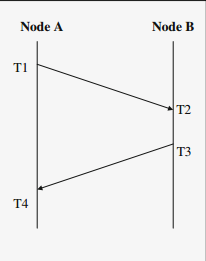
\includegraphics[height=6cm]{zigbee}
  \caption{ZigBee无线通信网络同步方法}
  \label{zigbee}
\end{figure}

\begin{equation}
%\left\{\begin{array}{l}
\begin{split}
&d = \frac{(T2 - T1) + (T4 - T3)}{2} \\
&\delta = \frac{(T2 - T1) - T3}{2}
\end{split}
%\end{array}\right.
\end{equation}

得到各个摄像头之间两两时间差后,即可根据时间差计算同步偏移量,实现系统同步。该方法实现较为简单,但应用前提是保持系统内网络传输延时固定,当网络状况发生变化时,摄像头之间的时间差计算就会出现误差。

第二种软件同步的方法是利用系统外部信号进行同步。这里的外部信号可以是计时器、灯光或者声音等多种可以被摄像头检测到的形式,当摄像头检测到这些信号后,以其作为基准点触发各个摄像头在预设好的时刻开始进行拍摄。

Shrestha等人在文献 \cite{shrestha2006synchronization} 介绍了一种外部信号同步方法,该方法利用闪光灯作为外部信号,在各个摄像头拍摄到的视频当中检测拍摄到闪光的那一帧,由于对于一次闪光,各个摄像头会在同一时刻捕捉到,因此根据闪光进行匹配即可同步时间。该方法主要分为两步:第一步是检测闪光,当某一帧图像拍摄到闪光时,图像的亮度直方图偏明亮的一部分会出现峰值,并且其相邻图像的亮度直方图中会出现低谷。因此在视频序列内按照此规律即可找到闪光灯所在帧。第二步是根据闪光对各个视频序列进行校准。如果将是否是闪光灯出现帧进行二值化表示,则各个视频序列可视为一个二进制向量,其互相之间的匹配问题就可以利用非精确字符串匹配实现。这个方法的同步精度同视频拍摄的帧率有关,误差为正负一帧。同时Shrestha等人在文献 \cite{shrstha2007synchronization} 中还介绍了以声音为同步依据的同步方法,匹配各个视频序列内的声纹信息,用以同步各个摄像头。

Jingyu Yan等人在文献 \cite{yan2004video} 中以时空兴趣点作为同步依据对摄像头进行同步。时空兴趣点是一种在视频图像中出现的,在时间和空间维度下都具有唯一性的特征点,并且在不同的拍摄角度下,这些特征点仍然不发生变化。这些特征点可以代表图像内物体的消失或者出现,物体的分裂或者合并以及物体运动速度的变化等等不同含义,通过设定不同的参数值选取图像当中最合适的的特征点,根据其分布情况进行匹配。

在文献 \cite{macmillan2015auto, schaffner2016vehicle} 中介绍了多摄像头系统同步在无人驾驶汽车上的应用,利用软件同步方法将汽车上装配的摄像头同步,实时采集车辆周围信息。

\section{本章小结}

本章介绍了多摄像头系统的相关研究现状,主要包括多摄像头系统的研究实例、同步控制方法和同步精度检测方法。目前多摄像头系统主要有两类实现方式,一类是大规模同类摄像头集成,可以利用较为低廉,性能一般的摄像头实现高性能摄像头的功能;一类是由异种摄像头组合搭配实现,针对系统的不同需求选取不同性能的摄像头组合搭配实现。多摄像头系统还有其他的实现方法,但其根本目的还是为了利用更多的易于获取的摄像头实现更高性能。

在搭建多摄像头系统的过程中,一个关键问题是如何解决同步问题。由于多摄像头系统需要各个摄像头之间在拍摄时间上受到精确控制,将摄像头进行同步即成为必不可少的环境。目前较为常见的同步控制方法可分为硬件同步和软件同步。硬件同步是指将各个摄像头通过硬件接口连接,由同步控制器发送同步信号控制各个摄像头的拍摄。这种方法虽然同步精度相对较高,但需要摄像头具有相应的硬件接口,对于摄像头的要求限制较多。另一种同步控制方法为软件同步,利用系统内的软件程序分析各个摄像头的拍摄时间并相应地进行调整,不断优化同步精度。这种方法适用于大多数摄像头,对于摄像头没有硬件限制,但是由于软件运行过程当中可能存在的网络延时、信号传输延时、程序运行延时、系统时间漂移等原因,会导致系统的同步精度降低,且这些误差随机存在,并不可控。

因此为了检测多摄像头系统的同步情况,需要对其进行拍摄时间检测。由于由系统为每帧拍摄图像设定的时间戳也可能存在误差,因此需要通过外部信号确定摄像头的拍摄时间。可以利用灯光、声音等信息作为检测信号,对摄像头的拍摄结果进行分析,确定真实的拍摄时间,最后进行匹配同步。这种方法能够有效排除系统内部误差干扰,检测系统的同步精度。
\chapter{数据库与测量分析}
\label{cha:database and measurement}

\section{引言}
由于本文主要研究的是演员在社交媒体上对电视剧的推广作用,涉及到电视剧、演员及微博信息。本章首先对电视剧及演员相关数据的数据库进行说明,然后对研究过程中需要的演员、电视剧、微博的特征及其提取过程进行介绍。之后对数据进行测量和分析,包括对微博影响力、话题热度、推广模式和他们之间的关系的研究和分析。

\section{数据集}
\subsection{数据库}
数据库系统包括演员数据库和电视剧数据库两部分,如图3.1。数据获取来源是爱奇艺\footnote{http://www.iqiyi.com/}、微博\footnote{http://www.weibo.com/}和豆瓣\footnote{http://www.douban.com/}。通过爬虫模拟登陆、模拟搜索的形式获取。

\begin{figure}[H] 
  \centering
  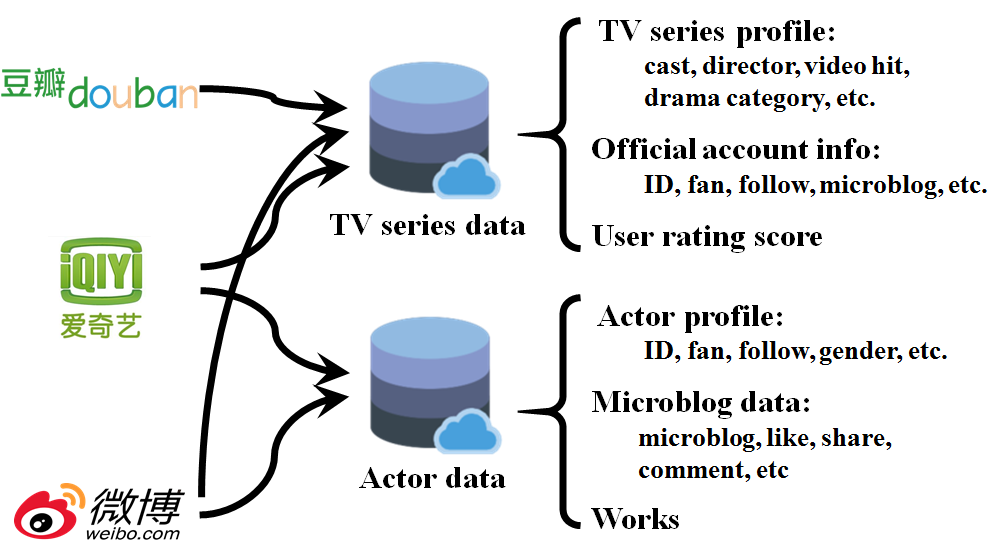
\includegraphics[height=4.5cm,width=8cm]{4}
  \caption{Data of the database}
  \label{4}
\end{figure}

爱奇艺是国内领先的视频网站,提供海量、优质的电视剧、电影、网络视频服务,网罗了中国最广大的年轻用户群体。爱奇艺打造涵盖电影、电视剧、综艺、动漫在内的十余种类型的中国最大正版视频内容库,也是中国付费用户规模最大的视频网站 \cite{http://www.iqiyi.com/common/aboutus.html}。爱奇艺数据爬虫获取爱奇艺电视剧页面每天的电视剧列表,然后访问每个电视剧的详情页,如图3.2,获得电视剧的相关信息,包括电视剧名称、主演、导演、类型、集数、播放量、简介等信息。

\begin{figure}[H] 
  \centering
  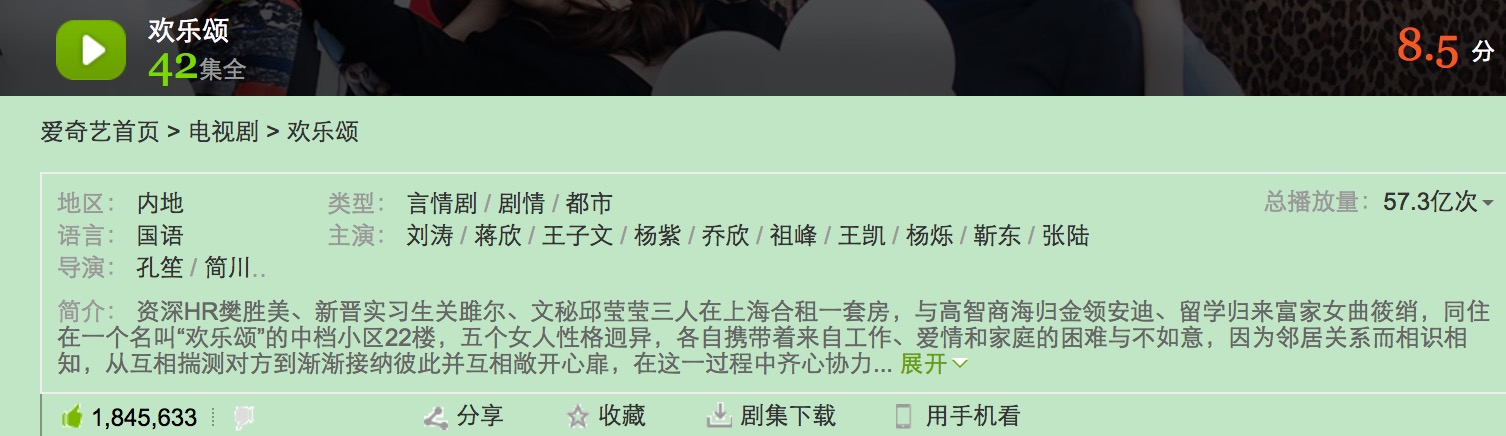
\includegraphics[height=4.5cm,width=8cm]{爱奇艺}
  \caption{电视剧欢乐颂详情页}
  \label{爱奇艺}
\end{figure}

豆瓣是一个社区网站,提供关于书籍、电影、音乐等作品的信息,无论描述还是评论都由用户提供(User-generated content, UGC),是中国Web 2.0网站中具有特色的一个网站\cite{https://zh.wikipedia.org/wiki/豆瓣}。对于电影和电视剧的豆瓣评分能反应当前广大群众对其质量、水平的认同情况。豆瓣爬虫根据爱奇艺爬虫获得的电视剧列表,从豆瓣搜索入口模拟搜索,获得该电视剧的豆瓣评分,以反应该电视剧的质量,如图3.3。

\begin{figure}[H] 
  \centering
  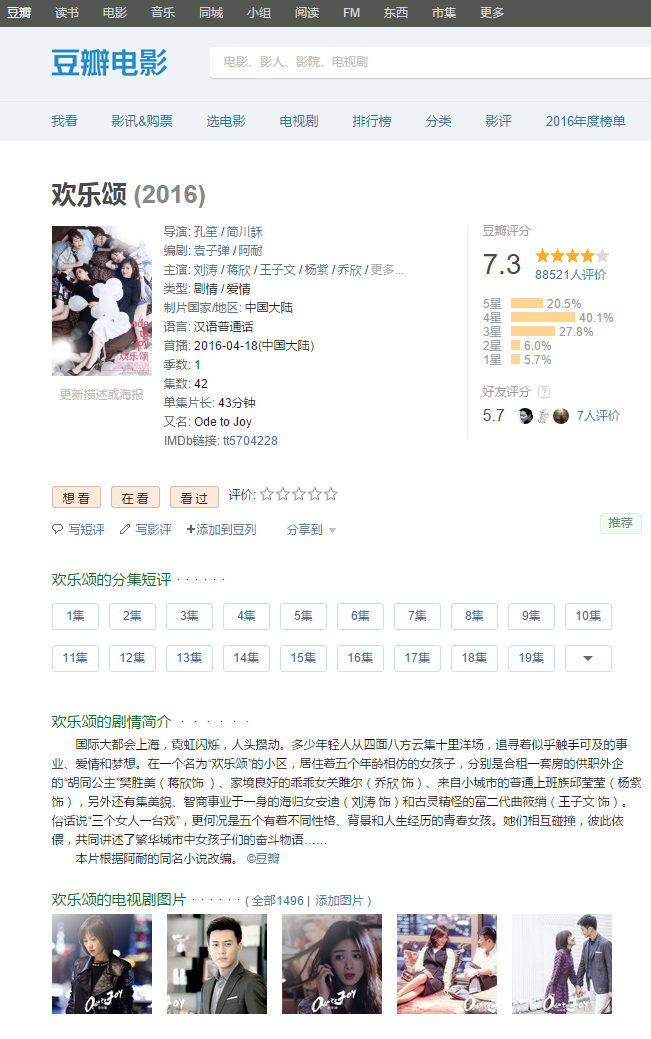
\includegraphics[height=4.5cm,width=8cm]{欢乐颂豆瓣}
  \caption{欢乐颂豆瓣主页}
  \label{欢乐颂豆瓣}
\end{figure}

微博是由新浪公司推出的提供微博客的服务网站。用户可以在微博网页、客户端发布140汉字(280字符)以内的信息,并可上传图片和链接视频,实现即时分享,同时,可以提供提供评论、转发、点赞功能。新浪微博是一个基于用户关系的信息分享、传播以及获取信息的平台,它占据中国微博用户总量的57\%,以及中国微博活动总量的87\%,是中国大陆访问量最大的网站之一 \cite{https://zh.wikipedia.org/wiki/新浪微博}。微博爬虫包括电视剧官方微博爬虫、电视剧话题爬虫和演员信息爬虫。

大部分电视剧在微博上都有官方微博,如图3.4,用来发布电视剧、演员相关的信息,比如电视剧预告、演员拍摄花絮、电视剧相关或者演员相关的推广信息等等,使得观众获得更多的关于电视剧和主演的信息和动态。电视剧官方微博爬虫根据爱奇艺爬虫获得的电视剧名称,获取电视剧在微博上官方微博的id,然后模拟访问主页,获得该电视剧官方微博的基本信息,包括id、粉丝数等,和发布的所有微博信息。

同时,大部分电视剧在微博上会有一到多个话题,以“\#话题名\#”的形式存在,如图3.5中欢乐颂话题主页,当用户在微博中发布微博讨论电视剧时会带上相关话题,使话题活跃。电视剧话题爬虫根据从电视剧官方微博中出现及微博搜索入口搜索电视剧名字,可以得到电视剧的话题名称,进而获得该电视剧话题的相关信息,包括话题阅读量、话题讨论量、话题粉丝量等。


\begin{figure}[H] 
  \centering
  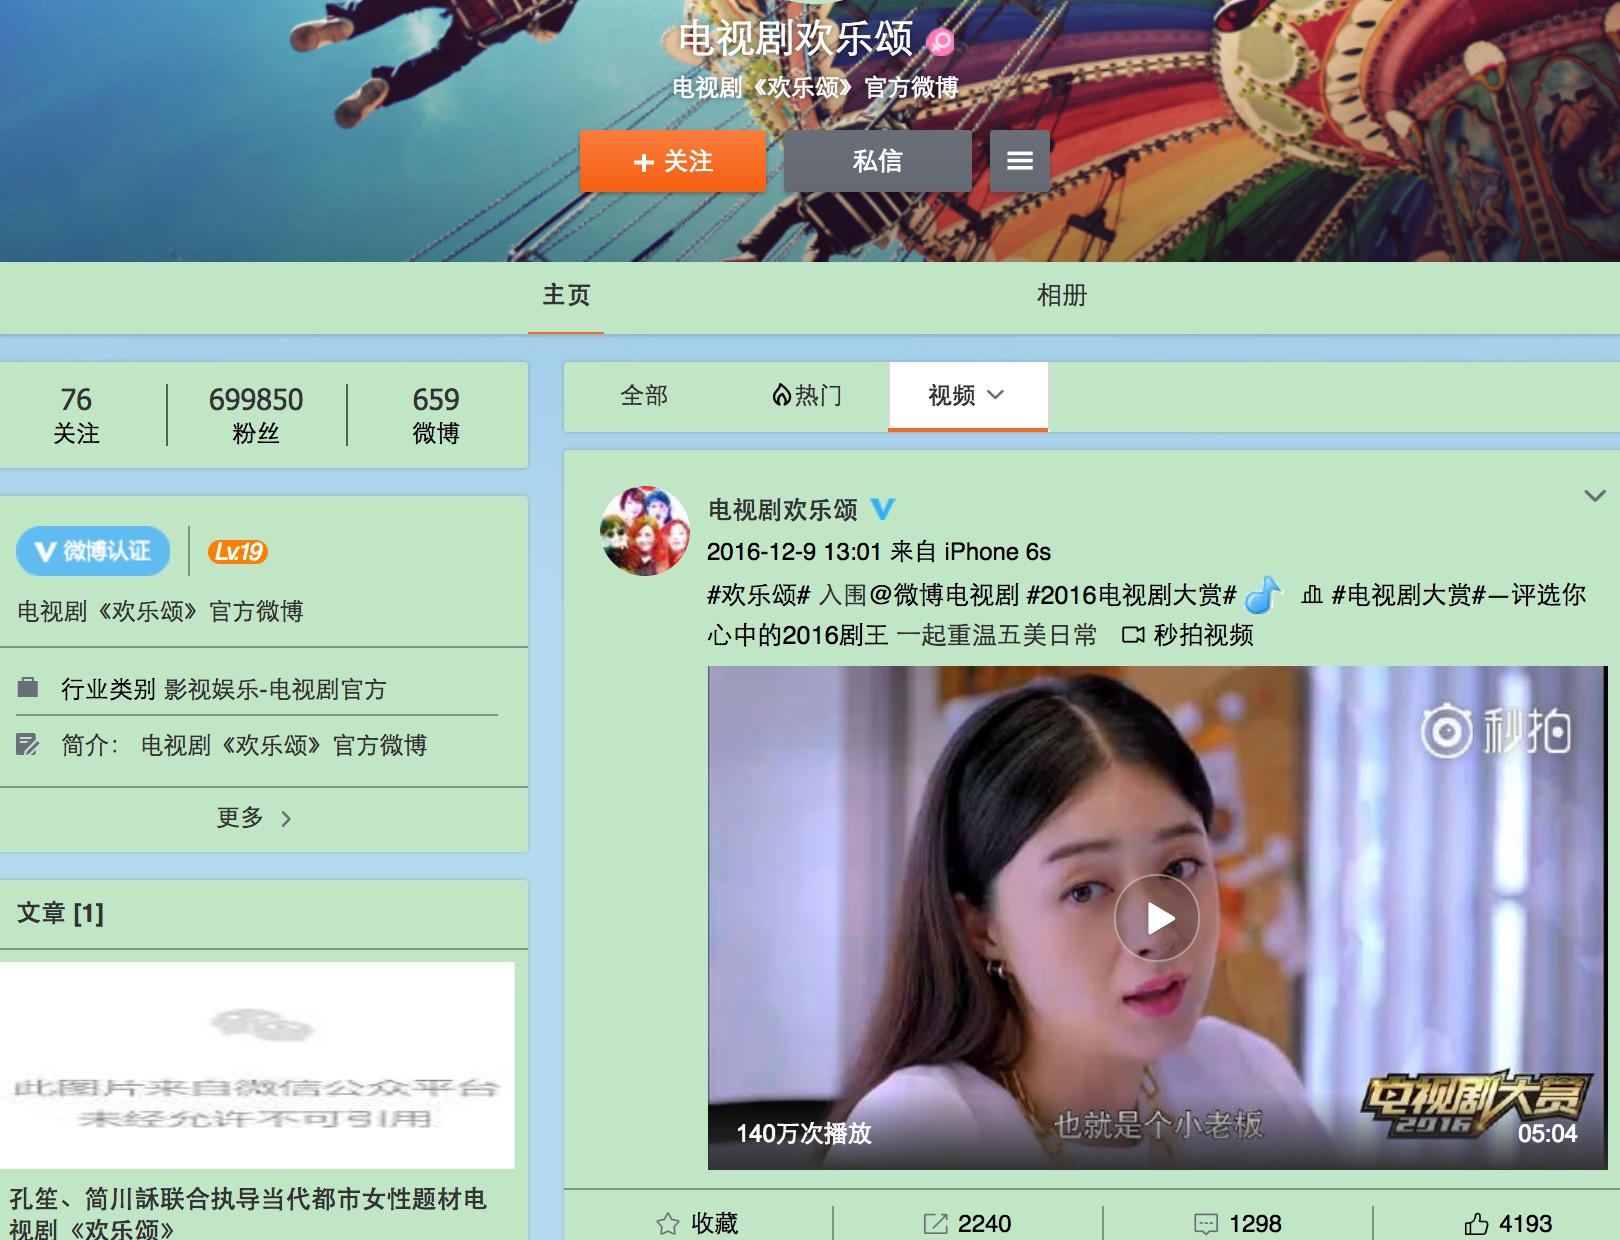
\includegraphics[height=4.5cm,width=8cm]{欢乐颂官微}
  \caption{电视剧欢乐颂官方微博}
  \label{欢乐颂官微}
\end{figure}
\begin{figure}[H] 
  \centering
  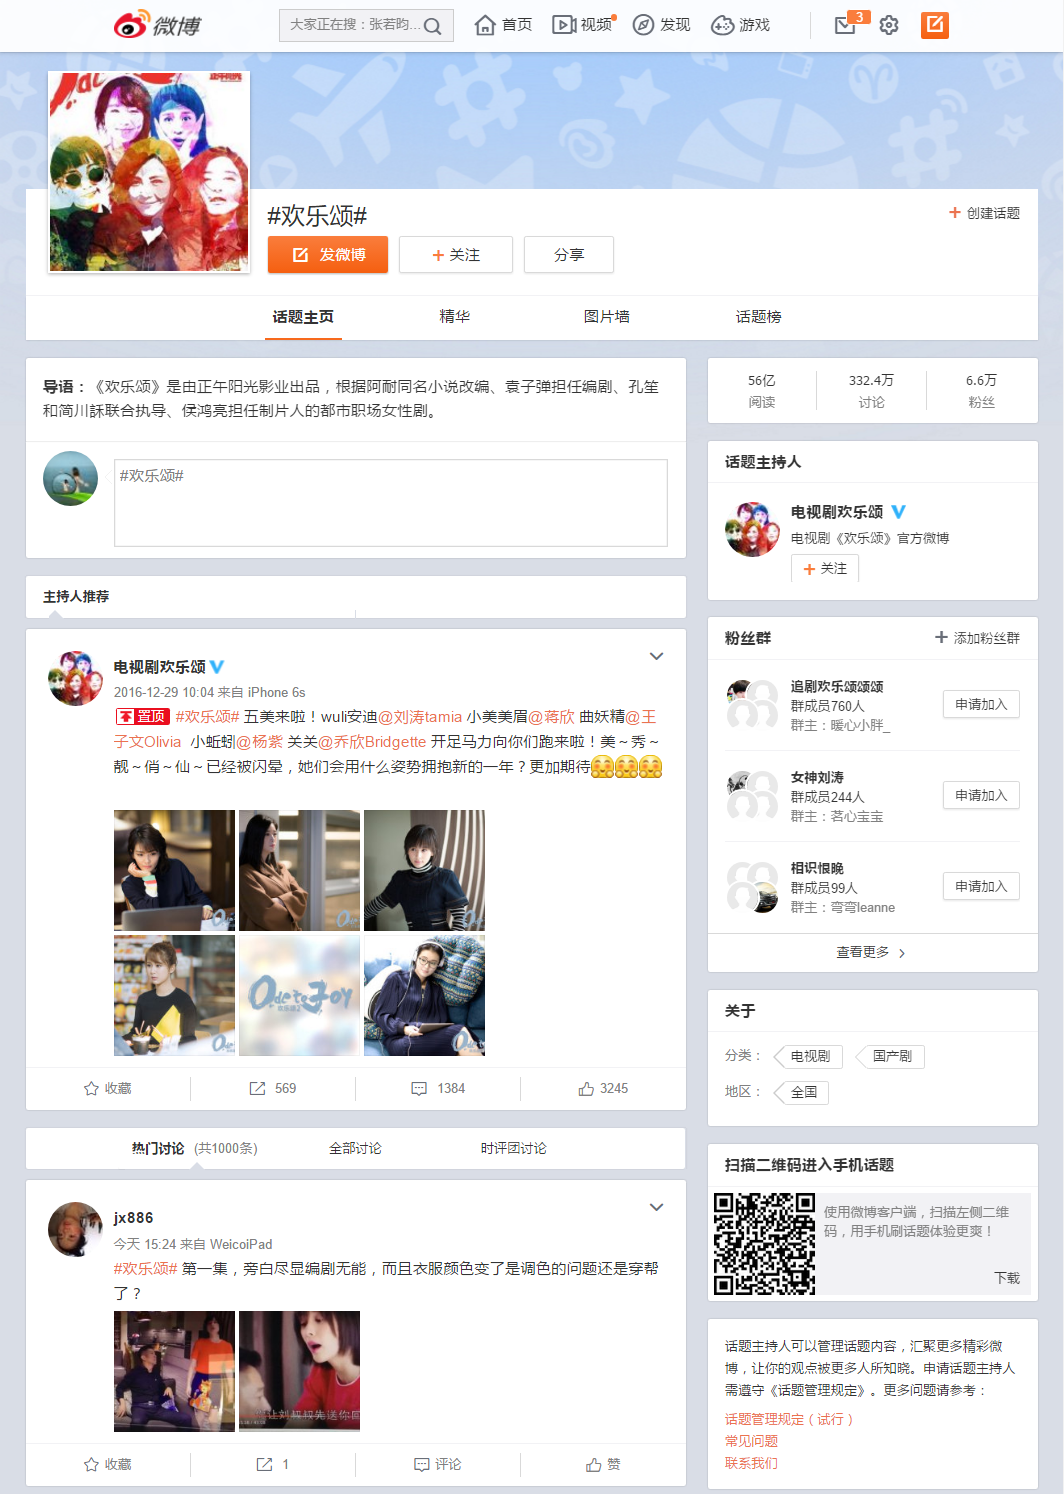
\includegraphics[height=4.5cm,width=8cm]{欢乐颂话题}
  \caption{电视剧欢乐颂话题主页}
  \label{欢乐颂话题}
\end{figure}

爱奇艺爬虫获取电视剧的主演后可以建成一个演员库,演员信息爬虫根据演员名字在微博上模拟搜索和百度搜索的形式获得演员微博上对应的id,然后根据id获得演员的基本信息和发布的所有微博信息,如图3.6。基本信息包括演员id、昵称、性别、描述、注册时间、粉丝数、关注数、微博数等等。微博信息包括发布的微博内容、时间及其获得的点赞数、转发数、评论数。

\begin{figure}[H] 
  \centering
  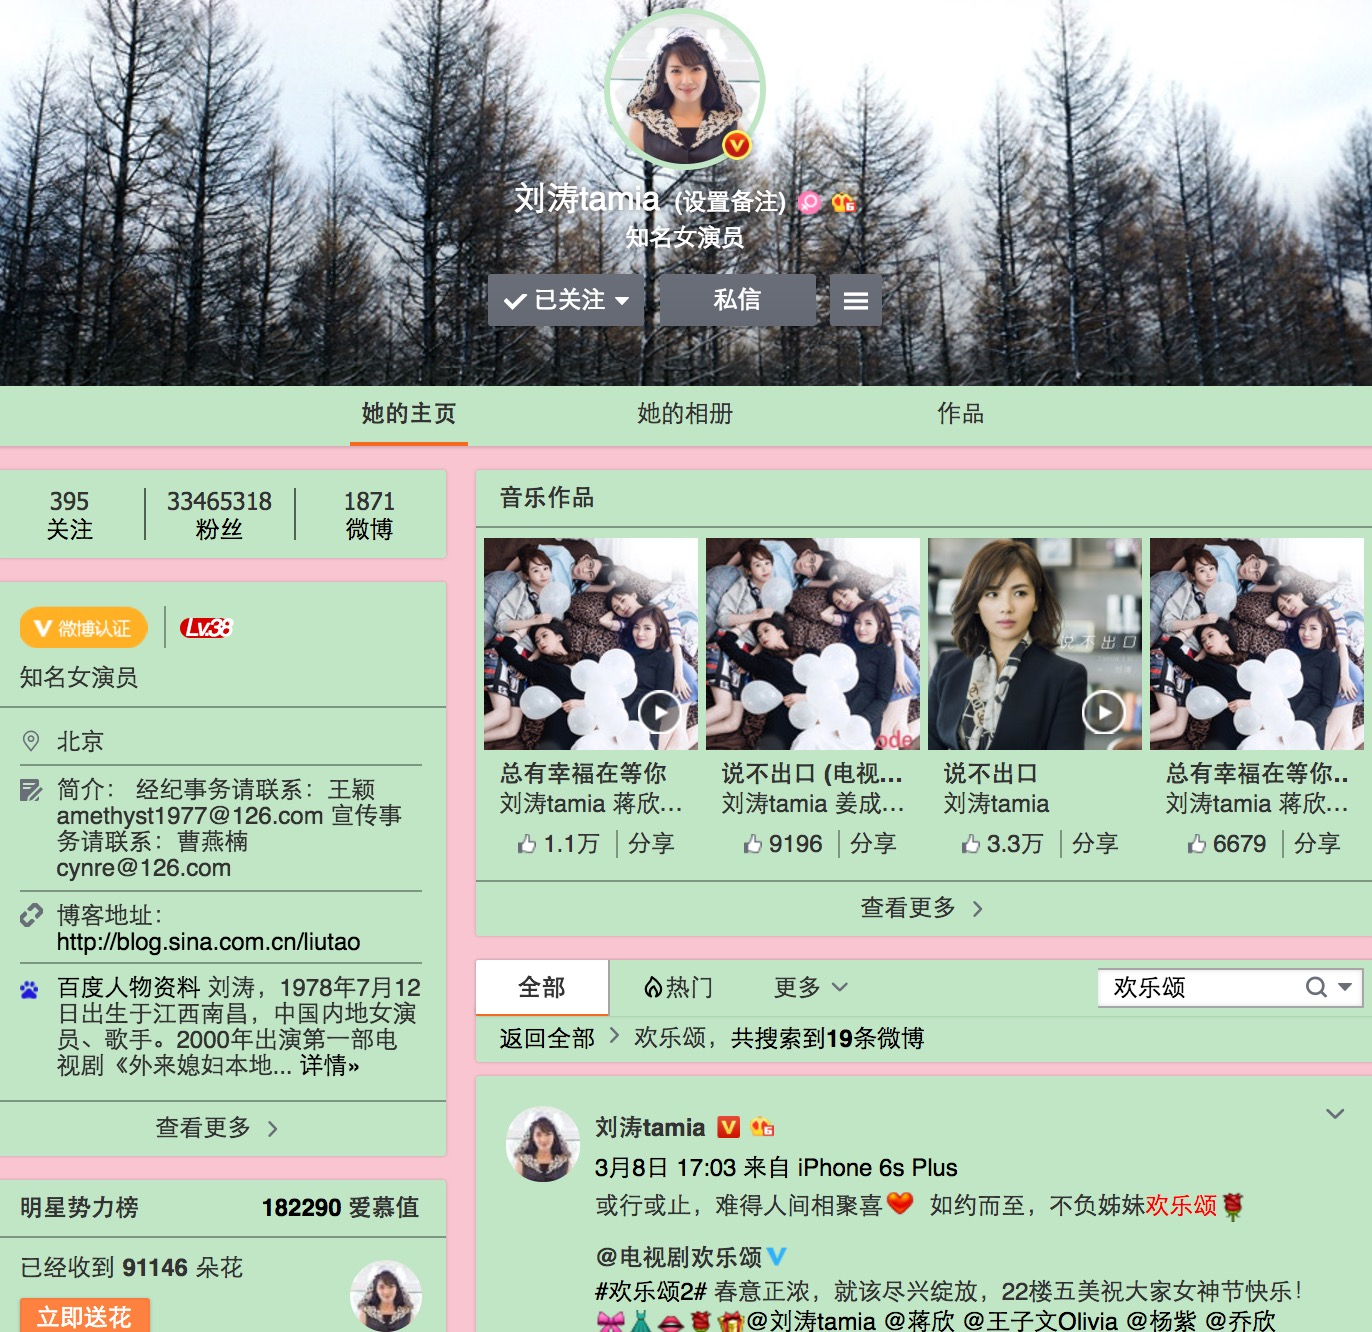
\includegraphics[height=4.5cm,width=8cm]{刘涛}
  \caption{刘涛微博主页}
  \label{刘涛}
\end{figure}

我们的爬虫运行在服务器后台,爱奇艺爬虫每天对电视剧信息进行爬取,微博爬虫每隔一段时间(3个月)从微博上对演员信息增量爬取。电视剧数据获取时间从2013年1月到2016年12月31日,微博爬虫全量获取演员信息和发布的微博信息。

\subsection{特征提取}
为研究演员所发微博的影响力,我们以微博作为研究对象,因此需要获得微博的基本特征。推广电视剧的微博有三方面的特征,一是来自发微博的演员的特征,包括演员粉丝数、性别和作品数。二是来自该微博推广的电视剧的特征,包括电视剧的豆瓣评分和演员阵容。三是来自微博自身的特征,包括该微博的发布时间、日期和内容。
发布微博的演员的特征中,粉丝数代表该演员在微博中粉丝量也就是影响力,当两个不同粉丝量的演员发布同一条微博时,粉丝量大的演员发布的微博会被更多的人看到,也就更容易起到更好的推广作用;男演员和女演员的行为本身有差异,其粉丝男女构成也有差异,相应的粉丝行为和对推广微博的行为也会有差异;演员的作品数代表该演员在影视界和群众视听中的活跃程度,演员出演的电视剧越多,越容易被观众记住也越有名。微博推广的电视剧的特征中,电视剧的豆瓣评分代表了看过的群众对该电视剧质量评价;电视剧的演员阵容用该电视剧所有主演的粉丝数的总和来表示,代表了这个电视剧整体的粉丝量和可能的受关注度,越多名人参与到同一部电视剧中,这个电视剧越容易火。微博自身的特征是由发布微博的演员决定的,包括时间、日期和内容,这是我们研究的主要内容。

\begin{figure}[!htbp]
\centering
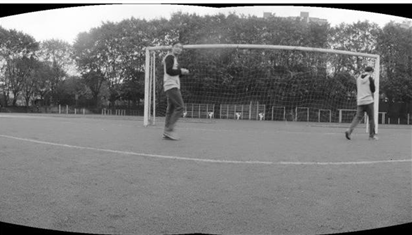
\includegraphics[height=5cm,width=8cm]{3}
\caption{Feature Extraction Module}
\label{3}
\end{figure}

对微博爬虫获取的微博,需要提取每一项微博的特征,因为微博自身的特征不需要从其他数据库或者爬虫获得,这里介绍前两方面特征的获取,如图3.7。对微博所推广电视剧的豆瓣评分从豆瓣爬虫爬取或者已爬取的数据库中搜索可得。该微博推广电视剧的微博的演员阵容,先从爱奇艺爬虫获取的电视剧信息中获得该电视剧的主演,然后从微博爬虫或者已爬取数据中获得这些演员的粉丝数目,求和得到阵容。发布微博的演员的作品数为统计爱奇艺爬取的所有电视剧中由该演员主演的数目。演员的性别由微博爬虫或已爬取的演员基本信息中获得。

\section{测量分析}
\subsection{微博影响力与话题热度}
(1) 微博影响力。
为了衡量一条微博的影响力,我们采用粉丝参与度作为评判标准,包括这条微博的转发数、评论数和点赞数,因为这些数据能反应看到并参与到电视剧推广中的用户数量。经过统计,所有演员的所有微博的转发数、评论数、点赞数的比例是${1: 1.86: 4.66}$,为了使这三项评判指标具有相同重要程度,因此赋予其权重比为${4.66: 2.51: 1}$,也能反应出转发、评论和点赞能带来的不同影响力。转发推广微博能使转发人的粉丝也看到,用户的参与感非常强,转发的人多了就具有滚雪球效应,能扩大宣传效果,因此其权重最大。用户通过评论推广微博参与到推广中,评论越多也越容易使该演员上微博热门,但评论并没有扩大用户群,所以用户参与感和影响力不如转发大。相比于转发和评论,用户点赞既不会扩大用户群也不需要输入文字,其用户参与感最弱,所以权重最小。定义微博影响力公式如下:
\begin{equation}P_i^j = 4.66 * W_p^i + 2.51 * W_v^i + W_a^i\end{equation}
其中,$P_i^j$ 表示与电视剧$j$相关的微博$i$的影响力,$W_p^i$, $W_v^i$和$W_a^i$分别表示微博$i$的粉丝转发数、评论数和点赞数。

那么对一部电视剧带来的微博影响力是它的所有主演的发布的推广微博的影响力之和:
\begin{equation}T_j = \sum_{i=1}^n P_i^j\end{equation}
其中$T_j$表示电视剧$j$所有主演的推广微博影响力之和,$n$为电视剧主演发布微博的数量。

(2) 电视剧微博话题热度。
我们研究的电视剧,每部在微博中都有对应的微博话题。每个微博话题都有相应的阅读量和讨论量,其中阅读量表示该话题的用户阅读数目,讨论量表示用户发布的带该话题名的微博数目。电视剧上映前和上映中进行宣传时,宣传方都会在发布微博时带话题发布,即带“\#话题名\#”的形式发布微博。话题讨论量和阅读量越多,表明越多的用户参与到该话题讨论中,越容易成为热门话题,进而达到更好的宣传效果。用户带话题名发布微博,会增加微博话题讨论量,使其粉丝看到该微博,提高微博话题阅读量。也就是说微博话题阅读量是话题讨论和宣传效果的体现,代表了该电视剧微博话题覆盖到的人数,是其热度的体现。因此我们选用电视剧的微博话题阅读量来衡量电视剧在微博中的话题热度:
\begin{equation}H_j = R_j\end{equation}
其中$H_j$表示电视剧$j$的微博话题热度,$R_j$表示微博话题的阅读量。

(3) 电视剧微博影响力与微博话题热度。
为检验电视剧微博影响力与话题热度的相关性,我们选用皮尔森相关系数(Pearson correlation coefficient)和最大信息系数(Maximal Information Coefficient, MIC)来检验。皮尔森相关系数可以反映出两个变量之间的线性相关程度,系数的变化范围为-1到1。系数值为1意味着变量X和Y呈完全正相关关系,Y随X增加而增加。系数值为-1意味着X和Y呈完全负相关关系,Y随X增大而减小。系数值为0意味着两个变量间没有线性关系。MIC是专门用于快速探索多维数据集的双变量依赖关系的度量。MIC是基于信息的非参数探索(MINE)统计方法系列的一部分,MINE不仅可用于识别数据集中的重要关系,还可用于表征数据集。MIC可以分析变量之间的广泛关系,而不限定于特定的函数类型\cite{10}。

\begin{table}[H]
\centering
\caption{Correlation between influence of microbloggings and topic hotness of TV series}
\begin{tabular}{|c|c|c|c|} \hline
variable x&varible y&PCC&MIC\\ \hline
influence&hotness&0.697&0.356\\
\hline\end{tabular}
\end{table}

经过统计,电视剧的微博影响力与最终话题热度高度相关,两者之间相关性如表1所示。因此,可以将微博影响力作为微博话题热度的评判标准,即在判断推广微博带来的营销效果时,推广电视剧的微博影响力大则说明该电视剧话题热度高。电视剧话题演化的和微博影响力的动态数据也验证了二者之间的相关性,以欢乐颂为例。电视剧微博话题热度与微博影响力每日变化如图,从图中可以看出,二者趋势和形状几乎一致。

\begin{figure}[!htbp]
\centering
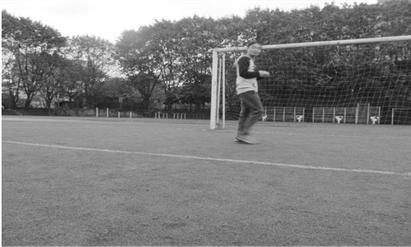
\includegraphics[height=3.cm,width=8cm]{1}
\caption{Everyday data of influence of microblogs and topic hotness}
\end{figure}



\subsection{推广模式}
(1) 推广周期。
演员对电视剧的推广周期主要可分为三个阶段,一是电视剧的筹备、拍摄阶段,二是电视剧首播阶段即第一集播出前后,三是首播之后的阶段,以电视剧“杉杉来了”为例,如图3.8。演员在电视剧拍摄期间会分享一些电视剧拍摄地、拍摄进度、角色和剧情相关信息等内容,这些微博不但可以让粉丝对演员的动态有所了解,还可以让观众提前了解电视剧相关信息,引起粉丝的兴趣和期待,起到提前宣传的作用。在第一集播放的前后几天是演员和电视剧官方宣传的高峰期,演员会发布微博进行大力度推广,我们将电视剧首集首播日前后5天定义为电视剧的首播阶段。统计发现虽然有些演员在微博中不活跃,但是仍然会在首播前后,发布微博进行推广宣传。首播阶段是影响收视率的关键时间,在这个时期演员推广可以提醒和号召粉丝看这个电视剧,促进提高话题热度和收视率。首播之后,演员还会继续进行微博推广,发布微博传递信息或者与粉丝互动,能在维持现有观众继续观看后续剧集的同时,吸引更多观众参与话题讨论并提高电视剧收视率。除此之外,当电视剧登陆其他电视台开播时,演员也会发布微博进行推广。因此,从推广周期来看,演员推广微博时期分为三类, 分别为筹备阶段、首播阶段和首播后阶段。
\begin{figure}[!htp]
\centering
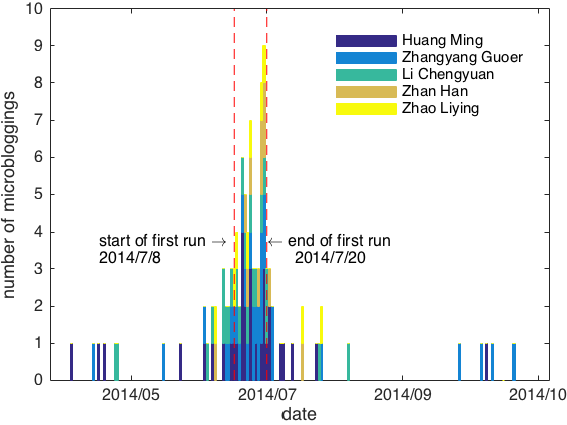
\includegraphics[width=7.8cm,height=4.5cm]{period}
\caption{Microbloggings distribution of different promotion period.}
\end{figure}

(2) 推广时间。
在一天中不同时间发布推广微博,由于用户使用习惯的差异,被用户看到的时长和概率不同,也就会达到不同的推广效果。比如同一条推广微博,在用户刷微博高峰和上班时间发布,肯定会获得不同的参与度。在一天中,午饭前、晚饭前及晚上通常都是用户刷微博的高峰时段。图3-8显示了演员发布微博时间的数目分布情况,同时也包括演员在电视剧上映前和上映后的数目差异。在本文中,我们想知道演员在不同时间段发布微博,哪个时间段会带来更好的推广效果,因此,我们将演员发布的微博根据发布时间分成三类,分别是上午(1时至12时),下午(12时至18时),晚上(18时至次日1时)。
\begin{figure}[!htbp]
\centering
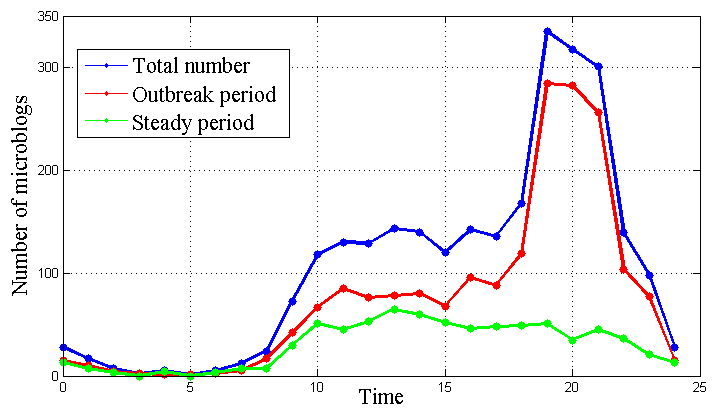
\includegraphics[height=3.5cm,width=8cm]{time}
\caption{Distribution of actors' microblogs along the time}
\end{figure}

(3) 互动模式。
在微博上推广电视剧过程中,演员会与其他主演、粉丝、电视剧官方微博等有很多交互行为来增加用户的参与度,促进电视剧的推广。图3-9展示了电视剧欢乐颂推广过程中出现的互动关系。图中每个节点表示一个演员或者官方微博账号,节点大小代表了与其他账号互动的数目,发过的微博中与其他账号互动越多,节点大小越大。有向箭头表明了互动的方向,边的粗细代表互动的频率,频率越高边越粗。一条微博可以使演员间、演员与官方微博间、演员与粉丝间建立互动关系,如图3-9中为一条微博的传播情况,图中黄色点是该电视剧的主演,每个点是一个微博用户,每条边是一个转发关系。

\begin{figure}[!htbp]
\centering
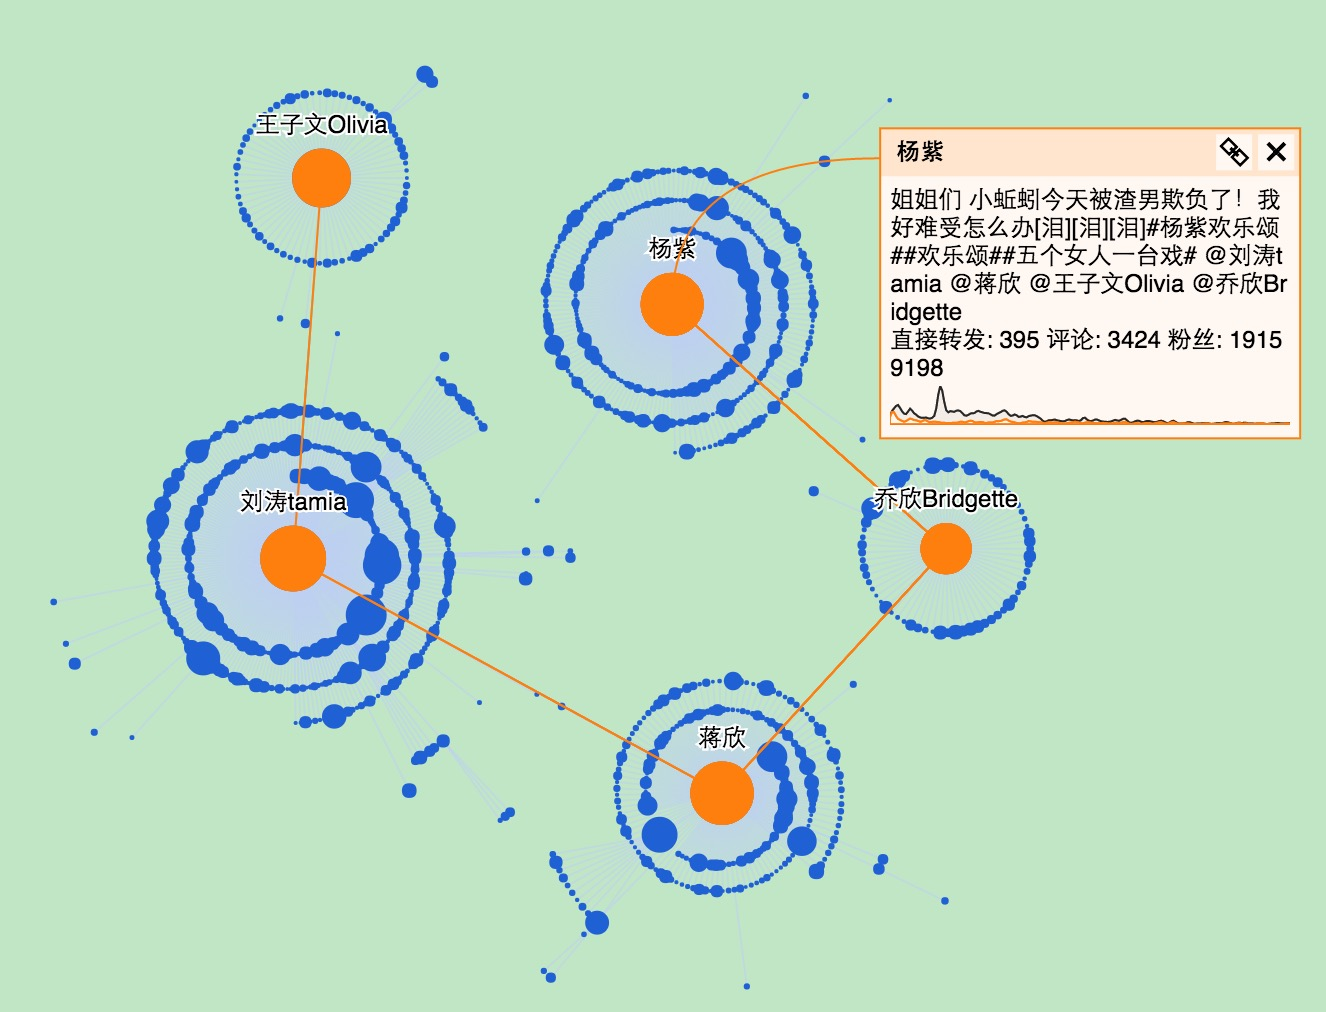
\includegraphics[height=4cm,width=5.4cm]{微博互动}
\caption{Interaction relationships of one microblog for TV series "\textit{Huanlesong}"}
\end{figure}

\begin{figure}[!htbp]
\centering
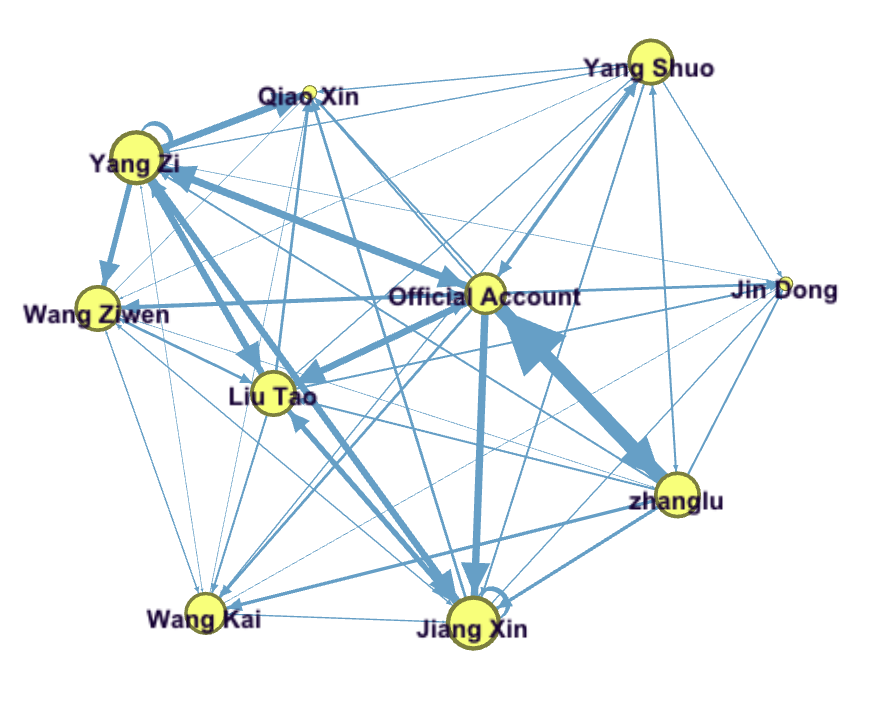
\includegraphics[height=4cm,width=5.4cm]{interaction}
\caption{Interaction relationships of TV series "\textit{Huanlesong}"}
\end{figure}

演员发布推广微博时有四种互动模式:
a. 与电视剧其他主演互动。演员会转发其他主演微博,或者发布微博“@”其他主演,在微博中与其他主要进行交流。主演间互动一方面会增加 微博话题性,另一方面也会结合多方粉丝,扩大推广效应。
b. 与官方微博互动。经过统计发现,一种常见的推广模式是,官方微博作为源头,发布推广微博,并在微博中“@”主演,主演将会转发这条微 博,提升官微推广的影响力。我们用累计分布图来分析演员响应官方微博的时间概率分布。以电视剧"\textit{欢乐颂}"为例,78\%的主演的响应时间在2小时以下。统计发现,对所有电视剧而言见图3-9,80\%的主演的响应时间都会在2小时以下。
c. 原创非互动微博。此类微博由演员原创, 虽然不包含与其他人的互动,但通过表达针对电视剧剧情或者人物的感想和看法,更好的表达演员的 情感和想法,更能够吸引粉丝的注意力。
d. 其他互动模式。除了以上三种互动的其他模式称为其他互动模式,包括演员转发视频网站官方微博的微博、转发粉丝微博、转发宣传媒体微博等。

图3-9显示了所有演员微博中以上四种模式所占比例,其中也包括了在电视剧上映前后的比例差异。

\begin{figure}[h]
  \centering%
  \subcaptionbox{TV series: "\textit{Huanlesong}"}[4.5cm] 
    {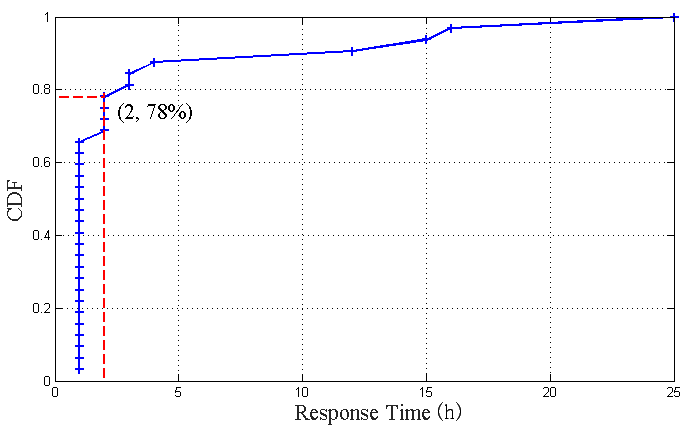
\includegraphics[height=3.7cm,width=7.5cm]{53}}%
  \hspace{4em}%
  \subcaptionbox{All TV series}[4.5cm] 
      {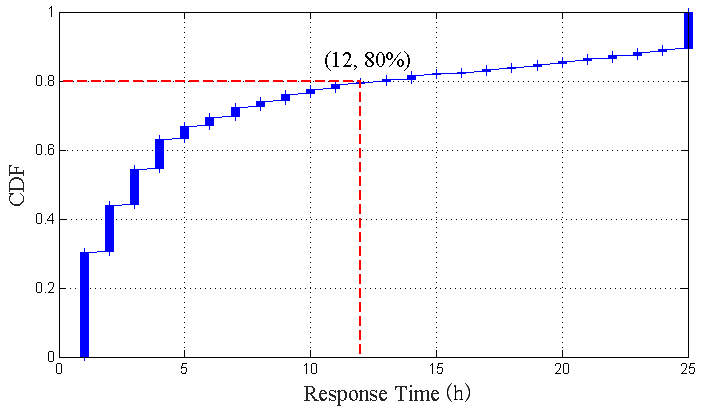
\includegraphics[height=3.7cm,width=7.5cm]{52}}
  \caption{Response time of actors to official accounts' references}
  \label{fig:big1-subcaptionbox}
\end{figure}

\begin{figure}[!htbp]
\centering
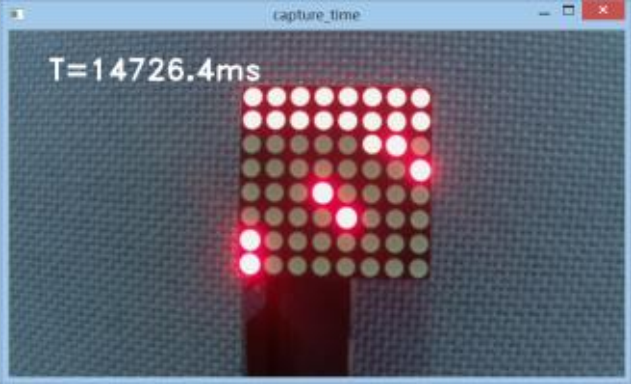
\includegraphics[width=8.5cm,height=3.7cm]{6}
\caption{Proportion of interaction modes}
\end{figure}

(4) 推广模式与话题热度。
为验证各种推广模式与话题热度的相关性,我们用皮尔森相关系数和最大信息系数来检验。通过两种检测方法可以表明各个推广模式与话题阅读 量具有较强的相关性,因此接下来我们就可以检验各个推广模式对话题热度的因果性和有效程度。
\begin{table}[!htbp]
\centering
\caption{The correlation between promotion patterns and topic hotness}
\begin{tabular}{|c|c|c|c|} \hline
\multicolumn{2}{|c|}{promotion patterns}&PCC&MIC\\ \hline
\multirow{3}{*}{promotion period} & preparation&0.389&0.284\\% \hline
&premiere&0.515&0.342\\% \hline
&post-premiere&0.813&0.399\\ \hline
\multirow{3}{*}{promotion time} &morning&0.239&0.306\\% \hline
&afternoon&0.542&0.407\\% \hline
&evening&0.856&0.340\\ \hline
\multirow{3}{*}{interaction mode} &actors&0.390&0.292\\% \hline
&official accounts&0.745&0.356\\% \hline
&original&0.600&0.297\\ 
&other&0.630&0.349\\ 
\hline\end{tabular}
\end{table}

\label{sec:multifig}


\chapter{演员社交推广行为的倾向值匹配算法}
\section{引言}
\section{数据处理}
\subsection{**数据清洗}
\subsection{混淆变量}
\subsection{推广策略}
\section{算法步骤}
\section{基于话题演化倾向值匹配}
\section{显著性及平衡性检验}
\section{本章小结}
\chapter{实验与结果分析}

\section{引言}

在本章,我们利用倾向值匹配算法对获取的数据进行实验分析,针对电视剧演员的不同行为模式进行比较,从而选取推广效果最好的推广策略推荐给演员,以求达到最好的宣传效果。首先,我们针对三种推广模式的十种推广策略,并引入演员的粉丝量作为混淆变量进行分析。通过分析结果可以看出,在首播后的阶段内,在早上发布更多的原创微博能够获得更好的推广效果。但是考虑到推广周期这一推广模式存在的问题,以及混淆变量数量过少对分析结果造成的影响,我们又提出了改进模型,对新获取的数据进行了新的实验。在改进实验中,将所有数据根据话题演化模型分为平稳期和爆发期两组,对于每组内的所有微博分析其推广时间和互动模式这两个推广模式的推广效果,并引入演员性别、电视剧评分等更多的混淆变量加入到模型当中,使得分析结果更具有可信性。同时我们还对分析结果进行了模型显著性检验和平衡性检验,验证了倾向值匹配算法的适用性和准确性。

\section{演员社交推广行为的影响力模型}

本节利用倾向值匹配算法,对演员发布的推广微博的影响力进行了建模,对不同的微博推广策略进行了对比,分析了不同推广策略所带来的不同的推广效果。

\subsection{实验数据}

本节选取爱奇艺和腾讯视频两个视频网站中,首次播放时间在2013年1月1日到2015年3月1日期间的222部电视剧作为研究对象。抓取电视剧的基本信息,包括电视剧主演、播时间、视频点击量等。同时在微博上抓取电视剧及其主演的微博数据。电视剧的微博数据包括电视剧相关微博话题的话题名称、话题阅读量、话题讨论量等;电视剧主演的微博数据包括222部电视剧所涉及的886个主演的个人信息和所发微博。其中个人信息包括演员的id、昵称、关注数、粉丝数、微博总数、注册时间以及演员的关注关系链等。演员所发微博数据包括所有发布的微博数目、内容、时间,以及每条微博下面的点赞数、转发数、评论数等信息,共计1671764条微博,其中与我们选定电视剧相关的有30959条微博。

\subsection{推广策略及混淆变量}

为研究演员社交行为对电视剧的推广作用,将演员发布的推广微博作为研究对象,根据3.3.2节的介绍,我们对三类推广模式下的10项推广策略进行研究,定义每一项推广策略为策略$t$,其取值为$T$。在我们的研究中,$T = {0, 1}$,其中$T = 1$代表采用这项策略,$T = 0$代表不采用这项策略。

\begin{table}[!htbp]
\centering
\caption{推广策略分类}
\begin{tabular}{|c|c|c|c|} \hline
\multicolumn{2}{|c|}{推广模式}&T=1&T=0\\ \hline
\multirow{3}{*}{推广周期} & 筹备阶段&筹备阶段发布&非筹备阶段发布\\% \hline
&首播阶段&首播阶段发布&非首播阶段发布\\% \hline
&首播后阶段&首播之后发布&非首播之后发布\\ \hline
\multirow{3}{*}{推广时间} &早上&早上发布&非早上发布\\% \hline
&中午&中午发布&非中午发布\\% \hline
&晚上&晚上发布&非晚上发布\\ \hline
\multirow{3}{*}{互动模式} &主演互动&与主演互动&非与主演互动\\% \hline
&与官微互动&与官微互动&非与官微互动\\% \hline
&原创&原创非互动&非原创\\ 
&其他互动&其他互动&非其他互动\\ \hline
\end{tabular}
\end{table}

当对某一项推广策略进行分析时,将其他策略视为混淆因素,加入混淆变量集合$X$。另外对于不同演员来说,其知名度和受欢迎程度对于推广微博的影响力有着很大的影响,更加流行的演员发布的微博能够收获更多的回复和点赞。而每个演员在微博上的粉丝数,是从侧面衡量演员流行度的一个指标。因此,我们将发布微博的演员的粉丝数同样作为一个混淆变量加入到模型当中,去除演员的粉丝数对分析结果的影响。由于不同演员的粉丝数量差别较大,有的著名演员拥有数百万的粉丝,而对于一些名气稍小的演员仅仅拥有几百或几千粉丝,因此为压缩粉丝数数据尺度,对各个演员的粉丝数取值为10的对数。

\subsection{算法应用}

根据第四章所介绍的方法,应用倾向值匹配算法对这些微博数据进行分析。

首先,对于要分析的每一项推广策略,可以将其他的推广策略视为混淆变量。那么对于全部待研究的十项推广策略来说,选取其中一项为研究对象,另外九项既为混淆变量,同时将演员的粉丝量也作为混淆变量,将其纳入逻辑斯地回归模型来计算每一条微博的倾向值。

然后,根据是否采用了这项策略,将所有计算出倾向值的微博分为两个样本集合,对两个样本集合中的微博根据其倾向值采用一对多匹配和基于卡尺的最近邻方法进行匹配。在基于卡尺的最近邻匹配过程中,经过对于实验数据的观察和分析,设置卡尺距离为0.09。

最后,计算平均干预效果ATT来衡量该项策略对结果的影响效果。用t-test来检验干预效果的显著性水平,即检验两组微博中的微博影响力水平是否有显著差异。

\subsection{结果分析}

通过倾向值匹配算法,得到针对不同推广策略的推广效果,可以更好地指导演员在社交网络上选择推广行为模式,提高电视剧收视热度。

\textbf{(1) 推广周期。}

按推广周期计算筹备阶段、首播阶段和首播后阶段的平均干预效果ATT如表~\ref{r1}所示。可以看到,在筹备阶段发布的微博的平均干预效果为负值,且t检验结果显著,说明筹备阶段发布的推广微博影响力不如非筹备阶段,即首播阶段和首播后阶段。而首播阶段发布微博的影响力效果虽然为负值,但是经过t检验,与非首播阶段发布微博的影响力效果没有显著差异。与二者相比,首播后阶段发布微博的影响力效果与筹备阶段和首播阶段相比有显著差异,会显著提高。分析原因可能是粉丝们在筹备阶段和首播阶段只能看到关于电视剧的少量信息和花絮,参与感较低,导致关注度不高;而当用户看过电视剧后,在演员利用微博进行电视剧推广时,粉丝们可以针对剧情、人物等积极参与讨论,对微博内容也可以有更多的态度和观点,此时进行推广,效果会更好。

\begin{table}[h]
\centering
\caption{推广周期策略比较}
\label{r1}
\begin{tabular}{|c|c|c|c|} \hline
推广周期 & ATT & 显著性\\ \hline
筹备阶段 & -674.204& 0.000\\ \hline
首播阶段 & -182.854& 0.260\\ \hline
首播后阶段 & 757.065 & 0.000\\ 
\hline\end{tabular}

\end{table}

\textbf{(2) 推广时间。}

计算各个推广时间干预效果ATT和t检验的结果如表~\ref{r2}所示。通过结果可以看出,三种推广时间策略都具有较高的显著性,但在早上发布微博的平均干预效果为正值,而其他两种策略的平均干预效果为负值。这说明,与想象中不同的是,早晨发布推广微博获得的推广效果要显著好于中午和晚上发布。原因可能是,推广信息具有时效性,对当天来说,早晨发布的微博一天中被看到的时长和概率是最大的,到了第二天,消息的时效性大大降低,导致粉丝的参与度大大降低。因此建议演员更多的在早晨发布推广微博。

\begin{table}[h]
\centering
\caption{推广时间策略比较}
\label{r2}
\begin{tabular}{|c|c|c|c|} \hline
推广时间& ATT & 显著性\\ \hline
早上 & 879.083& 0.000\\ \hline
中午 & -138.270& 0.036\\ \hline
晚上 & -314.376 & 0.000\\ 
\hline\end{tabular}

\end{table}

\textbf{(3) 互动模式。}

按互动模式将演员推广行为分为与其他主演互动,与官微互动,原创非互动和其他互动四种方式。经过倾向值匹配算法,得到结果如表~\ref{r3}所示。可以看到演员与其他主演互动、与官微互动和发布原创微博时,平均干预效果都有所增加,都对推广有显著效果。因为主演和主演互动本身就在制造话题性,与官微互动,会转发一些电视剧情节、花絮及与演员相关的信息,信息量较大,会增加粉丝参与。而原创非互动模式与非原创相比,平均干预效果显著提高,推广效果提高的最大。分析演员的微博可知,原创微博更能表达演员的情感和对粉丝参与的情感呼吁,因而更能得到粉丝的支持和参与,推广效果也会更好。与之对比,转发其他视频网站、粉丝的微博等其他互动方式的推广效果明显不如另外三种互动方式,不管从携带信息量还是从演员情感角度看,其他互动方式的宣传效果都会较差。

\begin{table}[h]
\centering
\caption{互动模式策略比较}
\label{r3}
\begin{tabular}{|c|c|c|c|} \hline
互动模式& ATT & 显著性\\ \hline
主演互动  & 759.315& 0.000\\ \hline
与官微互动 & 3413.222& 0.000\\ \hline
原创  & 12007.880& 0.000\\ \hline
其他互动 & -7195.497 & 0.000\\ 
\hline\end{tabular}
\end{table}

通过以上的实验结果可以看出,不同的推广策略能够带来不同的推广效果,利用倾向值匹配算分能够有效区分混淆变量对于因果分析的影响。但是在本节所介绍的实验中,我们仅仅将演员的粉丝量加入到混淆变量当中,即区分了演员不同的流行程度、人气指数对结果的影响。但是还有其他的众多因素能够影响推广效果,例如演员的性别、年龄、电视剧的演员阵容等,因此需要将更多的因素列入到混淆变量当中进行分析。同时,对于推广周期这一推广模式而言,由于大多数演员会在整个电视剧的宣传周期内持续发布众多的微博,虽然根据倾向值匹配的分析结果,在不同阶段发布的微博能够获得不同的推广效果,但这并不会影响演员发布推广微博的频率。而且通过对不同阶段发布的微博的分析可以发现,不同微博之间的内容、受关注程度等都存在较大差异,仅仅将其划分到不同的推广周期并不能清晰地体现出其中存在的差异。因此,并不应该将微博的推广周期视为一个较为合理的推广模式进行讨论。针对本节实验存在问题,我们提出了一种基于话题演化模型的改进方法,更好地对不同的推广模式进行了比较。

\section{基于话题演化的模型改进}

本节是对上一节应用的改进优化,使倾向值模型更合理的应用在演员推广行为的分析中。不但结合话题演化规律,将话题根据电视剧上映时间分成平稳期和爆发期,分别在两个时期分析演员的推广行为和推广策略,而且将更多会影响电视剧话题热度的因素考虑在内,使分析结果更具有可靠性。

\subsection{电视剧话题演化规律}

研究发现,微博热点话题在传播过程中,不仅关键词高度集中、受外界环境影响显著,而且传播具有周期性。话题周期一般包括话题发生、话题发展、话题高潮和话题消退四个阶段 \cite{赵龙文2013基于意见领袖参与行为的微博话题热度预测研究}。统计发现,电视剧微博话题演化符合话题演化的基本特征,具有一定的周期特性,如图~\ref{ning}所示,电视剧《柠檬初上》的话题发展正是经历了话题发生、话题发展、话题高潮和话题消退的过程。

在话题演化发展的过程中,“意见领袖”起到了重要的引导作用,他们在信息传播的网络中扮演了关键节点的角色,他们可以为其他人提供信息、传播态度,同时也起到了过滤作用,将其希望传播的信息传递给其他人,而将其不希望传播的信息截留在自身节点处。同样,在电视剧话题演化的过程中,演员就充当了意见领袖的作用,他们不仅拥有很庞大的粉丝群体,还有很大的社交影响力。他们发布的微博信息往往能受到高度关注,在电视剧话题发展过程中,演员发挥了核心作用。在电视剧话题发展过程中有三个重要时间节点导致了电视剧话题向下一阶段的发展,分别是电视剧上映时间确定、首集播出时间、首轮播出结束。在电视剧上映时间确定之前,演员会不时发些电视剧相关信息包括电视剧拍摄进度、拍摄期间趣事、角色定妆照等信息的微博,提前宣传使电视剧话题在微博产生。当电视剧上映时间确定后,主演通常都会发微博宣传电视剧,推动话题发展和酝酿,吸引粉丝和普通用户注意上映时间,吸引第一批群众。当电视剧首轮播放第一集之后,演员发布微博来吸引观看用户参与电视剧剧情、角色相关的讨论,用户也因为看过电视剧,在微博上更愿意参与到话题讨论中去,带来话题热度的大发展。演员和用户的这种行为会持续到电视剧首轮播放结束后几天,之后话题因为其时效性,最终走向消退。

\begin{figure}[!htbp]
\centering
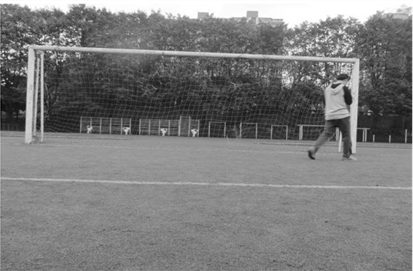
\includegraphics[width=9cm]{2}
\caption{电视剧《柠檬初上》的话题演化过程}
\label{ning}
\end{figure}

电视剧话题出现和发展期相对于话题爆发和消退期存在本质上的差别,即电视剧是否已经上映,带来用户对电视剧的内容了解的差异和参与方式的不同,进而导致话题热度发展不同。因此,本文中将电视剧话题根据电视剧是否上映分成两个主要时期,上映前为平稳期,上映后为爆发期。在电视剧话题的整个发展过程中,因为电视剧所处宣传期不同,演员在微博上不同时期的推广方式也会有差异。例如,对发布推广微博的时间,如图~\ref{time},在平稳期夜晚发布微博很少,白天不同时间发布微博数量比较平稳。但是在爆发期,在电视剧上映前后演员会有一个发布微博的高峰。在此时间发布微博不但能维持既有用户群观看电视剧、参与到电视剧话题讨论,还能吸引和号召新用户观看当天剧情。在不同时期演员发布推广微博的互动模式也有差异,从图~\ref{inter3}可以看出,与平稳期相比,爆发期演员会更多的与官方微博互动。因为当电视剧上映后,官方微博会发布更多的微博,包括剧情讨论、角色讨论、剧照、下集预告等等。

因此,研究演员在不同时期推广策略的有效性是非常有必要的。在本节,我们将演员发布的所有推广微博以电视剧上映的那一天作为时间节点,划分为两个时期分别进行讨论,即话题平稳期和话题爆发期。在各个时期内,利用倾向值匹配算法分析各个推广策略的推广效果。

\subsection{实验数据}

在本节,为了验证改进模型的可行性和准确性,我们又抓取了新的实验数据。通过爱奇艺爬虫,我们获取了2016年1月1日至2016年12月31日之间上映的所有电视剧和这些电视剧的所有主要演员姓名,一共有313部新的电视剧和1121位演员。根据这个电视剧名单,我们通过爱奇艺和豆瓣网站获取了这些电视剧的首播时间、观看量等数据。同时,在微博上获取了这些电视剧的话题数据、官方微博数据、主演数据。其中话题数据包括每天话题的讨论数和阅读数。官微和演员微博数据包括他们的基本信息和发布的所以微博信息,一共提取到了114767条微博。具体数据如表~\ref{data1}所示。

\begin{table}[!htbp]
\centering
\caption{实验数据}
\label{data1}
\begin{tabular}{|c|c|c|} \hline
数据集 & 数据名称 & 具体内容\\ \hline
\multirow{2}{*}{电视剧数据} & 豆瓣 & 豆瓣评分\\% \hline
& 爱奇艺 & 主演,首播时间,观看数\\ \hline
\multirow{3}{*}{微博数据} & 微博话题 & 讨论量,阅读量\\% \hline
& 官方账号 & 基本信息,微博\\% \hline
& 主演账号 & 基本信息,微博\\ \hline
\end{tabular}
\end{table}


\subsection{推广策略及混淆变量}

与上一小节相似,我们讨论推广时间和互动模式两个推广模式下的七种推广策略。而推广周期这一模式根据话题演化规律被分为平稳期和爆发期分别进行讨论,对分别属于这两个周期的所有微博进行倾向值匹配比较。

在倾向值匹配算法中,应该控制混淆变量使得混淆变量在策略组和非策略组分布相似,这样才能更好的分析策略的效果。考虑到影响一条微博在微博中热度的因素有很多,除了演员的推广策略本身,还受演员本身属性及电视剧属性等的影响,因此,本章中我们选用如表~\ref{mul}中包括演员和电视剧相关属性的信息作为混淆变量,使分析结果更具有可靠性。

\begin{table}[!htbp]
\centering
\caption{混淆变量}
\label{mul}
\begin{tabular}{|c|c|} \hline
种类 & 特征\\ \hline
\multirow{3}{*}{演员} & 粉丝数量\\% \hline
& 性别\\% \hline
& 作品数量\\ \hline
\multirow{2}{*}{电视剧} & 演员阵容\\% \hline
&豆瓣评分 \\ \hline
\end{tabular}
\end{table}

同样,在研究某一项推广策略时,将其他待研究的策略归为混淆变量,与以上介绍的这些混淆变量一起加入到混淆变量集合当中进行分析讨论。

\subsection{算法应用}

对于本实验来说,将倾向值匹配算法应用到实验数据上的方法与上一小节所介绍的实验类似。但由于采用了基于话题演化的模型改进,因此在开始进行分析之前,需要首先将所有微博根据发布的时间,以电视剧的首播时间为分割点,分为平稳期发布的微博和爆发期发布的微博两组,分别进行分析。

同时由于在本实验中,我们在社交网络上提取了更多的信息,也就可以在倾向值匹配模型中加入更多的混淆变量以更好地分析推广策略与推广效果之间的因果关系。而将这些混淆变量纳入逻辑斯地回归模型来计算每一条微博的倾向值的方法与上一节所介绍的方法相同。

然后,根据第3章所介绍的方法对已经得到倾向值的各个微博进行匹配,并对匹配结果计算平均干预效果来衡量该项策略对结果的影响效果。

\subsection{结果分析}

将倾向值匹配算法分别应用在演员推广的平稳期和爆发期,对各项推广策略进行因果分析,得到的推广策略有效性和t检验结果如表~\ref{res1}所示:

\begin{table}[!htbp]
\centering
\caption{基于话题演化模型的倾向值匹配结果}
\label{res1}
\begin{tabular}{|c|c|c|c|c|c|} \hline
\multicolumn{3}{|c|}{平稳期}& \multicolumn{3}{c|}{爆发期}\\ \hline
推广策略 & ATT & 显著性& 推广策略 & ATT & 显著性\\ \hline
早上 & -0.141 & 0.267& 早上 & 0.222 & 0.410\\% \hline
中午 & 0.023 & 0.837 & 中午 & 0.211 & 0.008\\% \hline
晚上 & 0.359 & 0.024 & 晚上 & -0.176 & 0.004\\ \hline
主演互动 & -0.088 & 0.561 &  主演互动 & -0.078 & 0.302\\
与官微互动& -0.318 & 0.002 & 与官微互动 & -0.001 & 0.989\\% \hline
原创& 2.633 & 0.000 & 原创& 1.860 & 0.000\\
其他互动& -0.743 & 0.000 & 其他互动 & -0.616 & 0.000\\ \hline
\end{tabular}
\end{table}

\textbf{(1)平稳期推广策略效果分析}

从表中可以看出,与在早晨和中午发布微博相比,在晚上发布微博的效果更好。用户晚上通常会花较多的时间在社交网络上,对他们而言,晚上发布的推广微博有更大的概率被他们看到。对互动模式而言,发布原创微博带来的推广效果要明显远远好于其他互动模式。与之相反,与官微互动和与其他人互动带来的推广效果较差。因为这种微博不能很好的表达演员自己的情感和想法,而且此时电视剧并未上映,粉丝参与电视剧推广微博更多的是因为演员,而不是因为剧情,因此对能更好表达演员自己想法和情感的原创微博会带来更好的粉丝参与度。与此同时,与其他主演互动的模式没有明显好的推广效果。

\textbf{(2) 爆发期推广策略效果分析}

在爆发期,下午发布的推广微博会带来更好的推广效果。在爆发期,演员通常在晚上会集中发很多微博,导致平均每条微博的粉丝参与度相对不高。从互动模式来看,发原创微博仍然是最有效的推广策略,原创微博需要演员投入更多的精力编写,同时更好的表达了他的想法和对粉丝参与的期望。而与其他人互动仍然效果最差,与官方微博和其他主演互动的推广效果并不显著。因此可知,在爆发期,演员在下午发布原创微博能获得更好的宣传效果。

\subsection{模型显著性及平衡性检验}

模型显著性及平衡性检验的作用是评估倾向值匹配模型是否恰当的进行了应用,对于待验证的各个策略来说,验证模型显著性即为验证所有混淆变量标准差在策略组和非策略组的平均值是否有显著差异,平衡性检验即为作累计分布图和分位数-分位数图(qq图)来看混淆变量在策略组和非策略组是否分布一致。表~\ref{res3}显示了两个时期,对于各个时间策略下,混淆变量的标准偏差。平稳期的标准偏差值在0.001到0.073之间,爆发期的标准偏差值在0.002到0.037之间,表明了策略组和非策略组的匹配样本的平均值分布一致。

\begin{table}[!htbp]
\centering
\caption{推广时间模式下,各个混淆变量的标准偏差}
\label{res3}
\begin{tabular}{|c|c|c|c|c|c|c|} \hline
&\multicolumn{3}{c|}{平稳期}& \multicolumn{3}{c|}{爆发期}\\ \hline
&早上&中午& 晚上 &早上&中午& 晚上\\ \hline
主演互动&0.012&0.073& 0.058&0.028&0.027& 0.008\\ \hline
与官微互动&0.029&0.007& 0.001&0.007&0.011& 0.003 \\ \hline
原创&0.053&0.006& 0.034&0.008&0.003& 0.008\\ \hline
其他互动&0.019&0.009& 0.047&0.018&0.006& 0.006\\ \hline
作品数量&0.006&0.023& 0.007&0.006&0.013& 0.007\\ \hline
性别&0.012&0.003& 0.054&0.023&0.047& 0.010\\ \hline
粉丝数量&0.008&0.033& 0.003&0.005&0.037& 0.002\\ \hline
演员阵容&0.012&0.033& 0.032&0.002&0.023& 0.003\\ \hline
豆瓣评分&0.030&0.049& 0.043&0.002&0.034&0.018\\ \hline
\end{tabular}
\end{table}

图~\ref{res2}显示的是在两个时期内,根据是否采用原创微博这条策略,绘制演员粉丝量、作品数、电视剧评分、电视剧阵容的累计分布图和分位数-分位数图,来刻画采用策略组和非采用策略组的混淆变量的分布情况。从图中可以看出,平稳期和爆发期的策略组和非策略组的这几个连续混淆变量的分布都非常类似。因此,倾向值匹配算法在我们的数据中得到了适当的应用,结果准确。

\begin{figure}[h]
  \centering%
  \subcaptionbox{平稳期\\.}
    {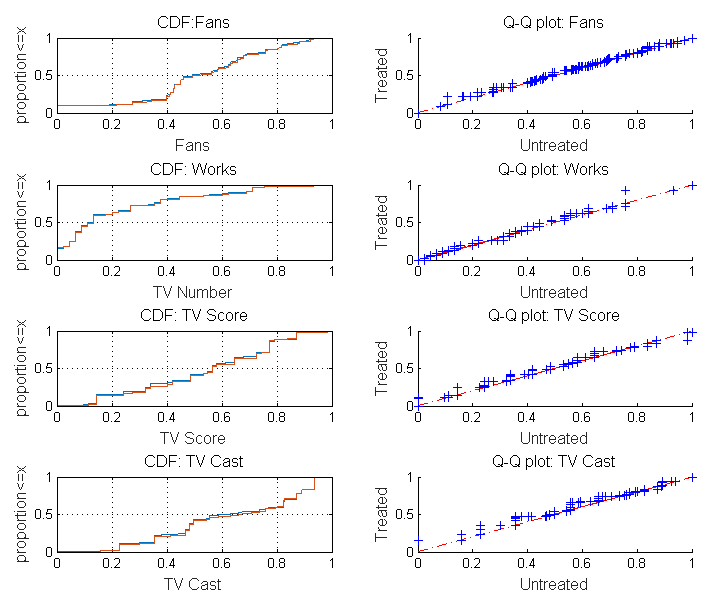
\includegraphics[width=12cm]{7}}
  \subcaptionbox{爆发期}
    {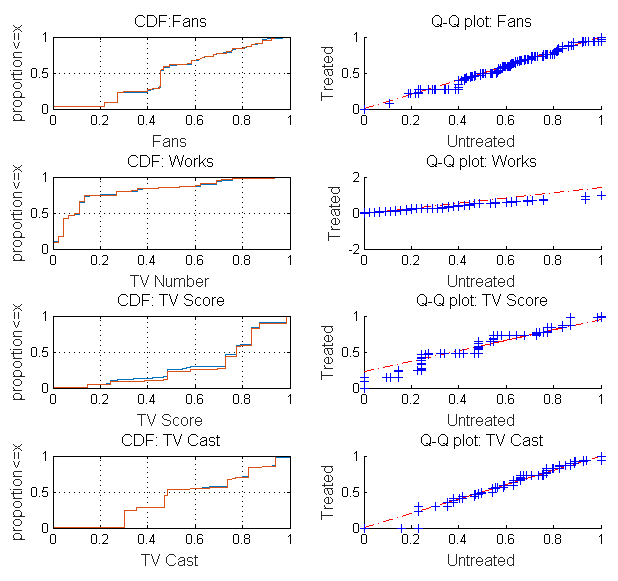
\includegraphics[width=12cm]{8}}
\caption{对于原创微博策略的平衡性检验}
\label{res2}
\end{figure}

\section{本章小结}

本章通过倾向值匹配算法对演员在微博上发布的推广微博进行了分析,针对不同演员不同电视剧的特点比较得出了最适合这个演员和这部电视剧的,具有最后推广效果的推广策略。在两组实验中,针对不同的演员和电视剧,通过倾向值匹配算法得到了不同的结论,比较得出了不同的最优推广策略,这充分验证的该算法对于不同比较对象所具有的针对性,利用该算法能够更有针对性地对演员的电视剧推广策略进行个性化的推荐,帮助其挑选出最优的推荐策略。




































\chapter{总结与展望}

\section{工作总结}

随着社交网络的不断发展,在微博、微信等社交媒体上进行宣传,已经成为一种重要的推广手段。尤其在电影宣传领域,越来越多的宣传方通过社交媒体推送广告,极大地促进了电影票房的增长。但是对于电视来说,由于其播放周期长、重复播放等特点,虽然同属于影视剧领域,但是与电影的宣传策存在一定的不同之处。因此,本文选取在微博上对电视剧的推广作为研究对象,比较不同的推广策略对最终推广效果的影响。

在微博上,主要是依靠电视剧官方账号和电视剧的主要演员创建与电视剧相关的话题,发布相关微博来进行推广。但是对于不同的电视剧和不同的演员来说,不同的推广策略能够获得的推广效果是不同的。同样的推广策略应用到不同的电视剧或者演员身上也会获得不同的效果。因此,在分析各个推广策略所获得的推广效果时,需要排除与电视剧和演员相关其他属性对结果的影响,仅仅分析策略和效果之间的直接关系。

因此,本文利用倾向值匹配算法来分析不同推广策略与推广效果之间的因果关系,将电视剧和演员信息作为混淆变量纳入模型当中,通过计算各个微博的倾向值,并对相同的倾向值进行匹配,从而可以找出成对的微博,每对微博之间的唯一差异在于是否采取了该项策略,而与其他因素无关。通过比较这对推广微博的影响力,就可以判断是否采取策略对推广效果所造成的影响。

同时,本文还根据电视剧话题在微博上的演化规律,提出了基于话题演化的改进模型,将所有微博以电视剧的首播日期为分界点,划分为平稳期和爆发期两组,对各组内的所有微博进行倾向值匹配,比较不同策略的推广效果。另外在改进模型中,还引入了更多的电视剧和演员的基本信息作为混淆变量,使得分析结果具有更强的因果关系。

本文通过网络爬虫,提取了2016年1月1日至2016年12月31日之间上映的313部电视剧和这些电视剧的1121位主演姓名,利用基于话题演化模型的倾向值匹配算法,分析推广时间以及互动模式两种推广模式与推广效果之间的因果关系。通过分析可以看出,在平稳期内,演员在晚上发布原创微博和在爆发期内,演员在下午发布原创微博能够获得更好的推广效果。并且通过进行模型显著性及平衡性检验,验证了该算法在数据集上实际应用的可行性和准确性。

\section{未来展望}

在后续工作中,为了验证算法的准确性,判断在分析过程当中是否忽略了某些信息,未能将其他与推广效果相关的信息纳入到混淆变量中进行讨论,还可以对结果进行敏感性分析,来判断各个推广策略对结果的影响程度。同时目前提取的关于电视剧和演员的社交网络数据还不算太多,在下一步的工作中,还可以进一步扩大数据获取来源,提取更多的电视剧以及演员信息,收集更多的微博数据,在更大的数据集下验证算法的准确性。同时,利用该算法还可以将收集到的数据整合成为一个建议系统,通过数据待推广的电视剧名称和要发布微博进行推广的演员名称,即可以根据电视剧和演员的自身特点,个性化地分析适合其的推广策略,帮助其选取推广效果最好的策略发布微博,使该方法具有一定的实用意义。

%%% 其它部分
\backmatter



% 参考文献
% 注意至少需要引用一篇参考文献,否则下面两行可能引起编译错误。
% 如果不需要参考文献,请将下面两行删除或注释掉。
\bibliographystyle{thuthesis}
\bibliography{ref/refs}


% 致谢
\begin{ack}

衷心感谢陶品老师对我的悉心教导,相识七载,亦师亦友,言传身教。在科研上,多少次迷茫困惑,是陶老师为我答疑解惑指点方向;在工作上,陶老师严谨细致吃苦耐劳的作风令我肃然起敬;在生活中,陶老师平易近人体贴入微,毫不吝啬对所有学生最真诚细致的关怀。师恩难忘,师道永记。

感谢孙立峰老师、杨士强老师对我的指导与帮助,感谢实验室的同学们方方面面的关心与照顾。

感谢我的父母和家人,虽然远在他乡,也能感受到他们时时刻刻对我的挂念。离开校园,也许更难再有时间回家看望,希望父母和家人一切安好,身体健康,平平安安。

感谢我的女友一萍,两年的朝夕相伴带给我无尽的欣喜、幸福与憧憬,感谢命运的眷顾让我们有幸遇见,待你我皆皓首,再相伴重温此文。

感谢清华,为我们提供了优异的学习、生活环境,只是数载科研鲜有成绩,愧对母校。吾校庄严,巍然中央。

\end{ack}



% 个人简历
\begin{resume}

  \resumeitem{个人简历}

  1991 年 1 月 6 日出生于山东省栖霞市。

  2010 年 9 月考入北京邮电大学计算机系,2014年 7 月本科毕业并获得工学学士学位。

  2014 年 9 月免试进入清华大学计算机科学与技术系攻读硕士学位至今。

  \researchitem{发表的学术论文} % 发表的和录用的合在一起
% 学位论文写作指南:
% 在学期间发表的学术论文分以下三部分按顺序分别列出,每部分之间空 1
% 行,序号可连续排列
% 1. 已经刊载的学术论文(本人是第一作者,或者导师为第一作者本人是第二作者)
% 2. 尚未刊载,但已经接到正式录用函的学术论文(本人为第一作者,或者
% 导师为第一作者本人是第二作者)。
% 3. 其他学术论文。可列出除上述两种情况以外的其他学术论文,但必须是
% 已经刊载或者收到正式录用函的论文。
  \begin{publications}
  \item 阎一萍, 姚鑫,孙立峰. 电视剧演员的社交推广行为的影响力模型. 第二十五届全国多媒体技术学术会议, 2016
  \item Yiping Yan, Lifeng Sun, and Xin Yao. Evaluating Actors' Promotion Behaviors for TV Series on Social Networks. Proceedings of the International Conference on Internet Multimedia Computing and Service. ACM, 2016.
  \item Yiping Yan, Lifeng Sun, and Xin Yao. How to Promote TV Series? Evaluating Actors’ Behavior on Social Media. The Third IEEE International Conference on Multimedia Big Data, Best Student Paper, 2017
  \end{publications}

\end{resume}

\end{document}
